%\noindent
\justifying
\setlength{\parskip}{1em}

In this chapter, the experiments conducted in this thesis are described along with evaluation metrics and results. In section \ref{EvaluationMetrics} the evaluation metrics like accuracy, precision, recall, confusion matrix, and f1-score are explained. These metrics are used to evaluate the domain gap between the distributions and quality of \ac{CycleGAN} generated document images. In section \ref{experiments} conducted experiments are explained along with training plots, confusion matrices, and classification reports. Finally, in section \ref{results}, quantitative and qualitative results are discussed thoroughly along with the typical failure cases.

\section{Evaluation Metrics}\label{EvaluationMetrics}

%\subsection{Accuracy}
%\subsection{Precision and Recall}
%\subsection{f1-score}

In machine learning research, numerous performance metrics have been introduced for neural networks. Each of which evaluates different aspects of neural network's performance. Hence, we need a specific set of performance metrics for a particular problem solved using neural networks. It's important to evaluate the performance of the neural network after training, using testing data, to determine its actual performance or generalization error on unseen data. Hence, the performance of classifiers trained upon different data distributions determined using annotated real document images (test dataset). The popular classifier performance evaluation metrics are accuracy, precision, recall, confusion matrix, and f1-score \cite{powers2020evaluation}. The testing dataset used to evaluate the classifiers is unbalanced, hence metrics like weighted average and macro average f1-scores are essential for the performance comparison of the classifiers trained on different data distributions. 

The accuracy is the most common metric used to evaluate classifiers. It is the ratio of accurately classified data items to the total number of observations (equation \ref{accuracy}). The precision is ``how many selected items are relevant". ``To put it another way, out of the observations that an algorithm has predicted to be positive, how many of them are actually positive" \cite{vakili2020performance}. The precision is the ratio of the number of true positives divided by the sum of the true positive and false positives (equations \ref{precision}). The recall is ``how many relevant items are selected". ``In fact, out of the observations that are actually positive, how many of them have been predicted by the algorithm" \cite{vakili2020performance}. The recall is the ratio of the number of true positives divided by the sum of true positives and false negatives. In below equations \ref{accuracy}, \ref{precision}, and \ref{recall} the $TP$ means true positives, $TN$ means true negatives, $FP$ means false positives, and $FN$ means false negatives.



\begin{equation}\label{recall}
\textit{Recall} = \frac{TP}{TP + FN}
\end{equation}

\begin{equation}\label{precision}
\textit{Precision} = \frac{TP}{TP + FP}
\end{equation}


\begin{equation}\label{accuracy}
\textit{Accuracy} = \frac{TP + TN}{TP +TN+ FP + FN}
\end{equation}

The f1-score is the harmonic mean of the precision and recall (equation \ref{f1-score}). The weighted average f1-score is determined by first calculating the f1-score of each class separately and each multiplied by the weight (the number of true instances for each class) and finally added together, hence favoring the majority class. The equation \ref{Weightedf1-score} represents the weighted average f1-score. The macro average f1-score computes the unweighted mean of separate f1-score of each class. The macro average f1-score does not take label inbalance into account. This leads to bigger penalization when the classifier does not perform well on minority classes. The equation \ref{macrof1-score} represents the macro average f1-score. In equations \ref{Weightedf1-score} and \ref{macrof1-score}, $N$ represents number of classes. More information about accuracy, precision, recall, and f1-score can be found \href{https://en.wikipedia.org/wiki/Precision_and_recall}{here\footnotemark.}
\footnotetext{\url{https://en.wikipedia.org/wiki/Precision_and_recall} last access: \dcdate}


\begin{equation}\label{f1-score}
\textit{f1-score} = \frac{2 \times precision \times recall}{precision + recall}
\end{equation}


\begin{equation}\label{macrof1-score} 
\textit{Macro average f1-score} =  \frac{f1_{class1} + f1_{class2}+ ... + f1_{classN}}{N}
\end{equation}


\begin{equation}\label{Weightedf1-score} 
\textit{Weighted average f1-score} =  \frac{f1_{class1} \times W_1 + f1_{class2} \times W_2 + ... + f1_{classN} \times W_N}{N}
\end{equation}



The confusion matrix is the most intuitive metric to determine the accuracy of the classifiers. It is useful when the classifier has to classify more than two classes. A confusion matrix is a table that describes how well a classifier performs on a test dataset that is labeled or annotated. The instances of the true class are represented at each row of the confusion matrix whereas the instances of predicted class probabilities are represented by each column or vice versa. Here, the confusion matrix is extensively used to analyze the performance of the classifiers trained on different data distributions. More information about the confusion matrix can be found \href{https://en.wikipedia.org/wiki/Confusion_matrix}{here}\footnotemark.
\footnotetext{\url{https://en.wikipedia.org/wiki/Confusion_matrix} last access: \dcdate}


\section{Experiments}\label{experiments}


In this thesis, several experiments were performed to understand the domain gap between data distributions. Three data distributions are considered for the experiments. Each data distribution represents a different domain. The synthetic document images represent the synthetic data distribution. The faxified document images represent faxified data distribution. The \ac{CycleGAN} generated images represent \ac{CycleGAN} generated data distribution. The goal of the experiments is to illustrate and analyze the domain gap between the real data distribution and above mentioned three data distributions. Also, one of the experiments was performed to determine the quality of \ac{CycleGAN} generated document images compared to the real document images. Now let's begin with the description of the experiments. First, the classifier(table \ref{table:ClassifierArchitecture}) is trained on synthetic document images and its performance is evaluated on annotated real document images. Second, the new classifier with the same architecture is trained on faxified document images and its performance is evaluated on annotated real document images. Third, the \ac{CycleGAN} is trained using synthetic document images and real document images and at the end of every epoch, the checkpoint is saved. As mentioned in training details \ref{TrainingDetailsCycleGAN}, \ac{CycleGAN} is trained for 20 epochs. 

Once training is finished, the latest saved checkpoint can be loaded to generate or transform images. The \ac{CycleGAN} trained considering synthetic data distribution as a source domain and real data distribution as a target domain. This means the synthetic document images represent the source domain and real document images represent the target domain. Next, the latest checkpoint is loaded, as we only need a generator $G$ to transform images from the source domain to the target domain. Hence, generator $G$ is retrieved to transform 100,000 synthetic document images into 100,000 realistic document images. We call these realistic document images as \ac{CycleGAN} generated document images which represents \ac{CycleGAN} generated data distribution. Further, 100,000 \ac{CycleGAN} generated document images are used to train another new classifier with the same architecture as the previous, and its performance is evaluated on annotated real document images. The experiment aims to understand the quality of the images generated by \ac{CycleGAN}. Especially, how efficiently \ac{CycleGAN} was able to close the domain gap between synthetic data distribution and real data distribution by generating quality images using generator $G$ in \ac{CycleGAN}. The evaluation metrics like accuracy, weighted average f1-score, and macro average f1-score \cite{lipton2014thresholding} are used to understand the contrast between the performance of the classifiers using annotated real document images.

\subsection{Experiment Steps}


\begin{enumerate}
    \itemsep0em 
    \item Train a classifier on synthetic document images and evaluate its classification performance on the annotated real document images.
    \item Train a classifier on faxified document images and evaluate its classification performance on the annotated real document images.
    \item Train a \ac{CycleGAN} using synthetic document images and real document images.
    \item Generate realistic document images using generator $G$ from the trained \ac{CycleGAN} model.
    \item Train a classifier on \ac{CycleGAN} generated realistic document images and evaluate its classification performance on the annotated real document images.
    \item Compare the classification performance of the above three classifiers on the annotated real document images, to illustrate the domain gap between real data distribution and other three distributions like synthetic data distribution, faxified data distribution, and \ac{CycleGAN} generated data distribution. The performance evaluation of a classifier trained upon \ac{CycleGAN} generated data distribution using annotated real document images describes, how close is the \ac{CycleGAN} generated data distribution to the real data distribution. Simply this approach determines the quality of the \ac{CycleGAN} generated document images compared to real document images.
\end{enumerate}


\subsection{\ac{CycleGAN} Training}

The image-to-image translation application, which is implemented using \ac{CycleGAN} is trained for 20 epochs and with batch size 1. For more \ac{CycleGAN} training details refer section \ref{TrainingDetailsCycleGAN}. The \ac{CycleGAN} consists of two generators $G$ and $F$. Along with two discriminators $D_X$ and $D_Y$. Domain $X$ represents the source domain and domain $Y$ represents the target domain. The developed image-to-image translation application aims to transform synthetic document images into realistic document images. Hence, the synthetic document images represent the source domain and real document images represent the target domain. The complete architecture of the image-to-image translation application using \ac{CycleGAN} is illustrated in figure \ref{fig:GxyFyx}.

\begin{figure}[H]
  \centering
  \begin{minipage}[b]{0.49\textwidth}
    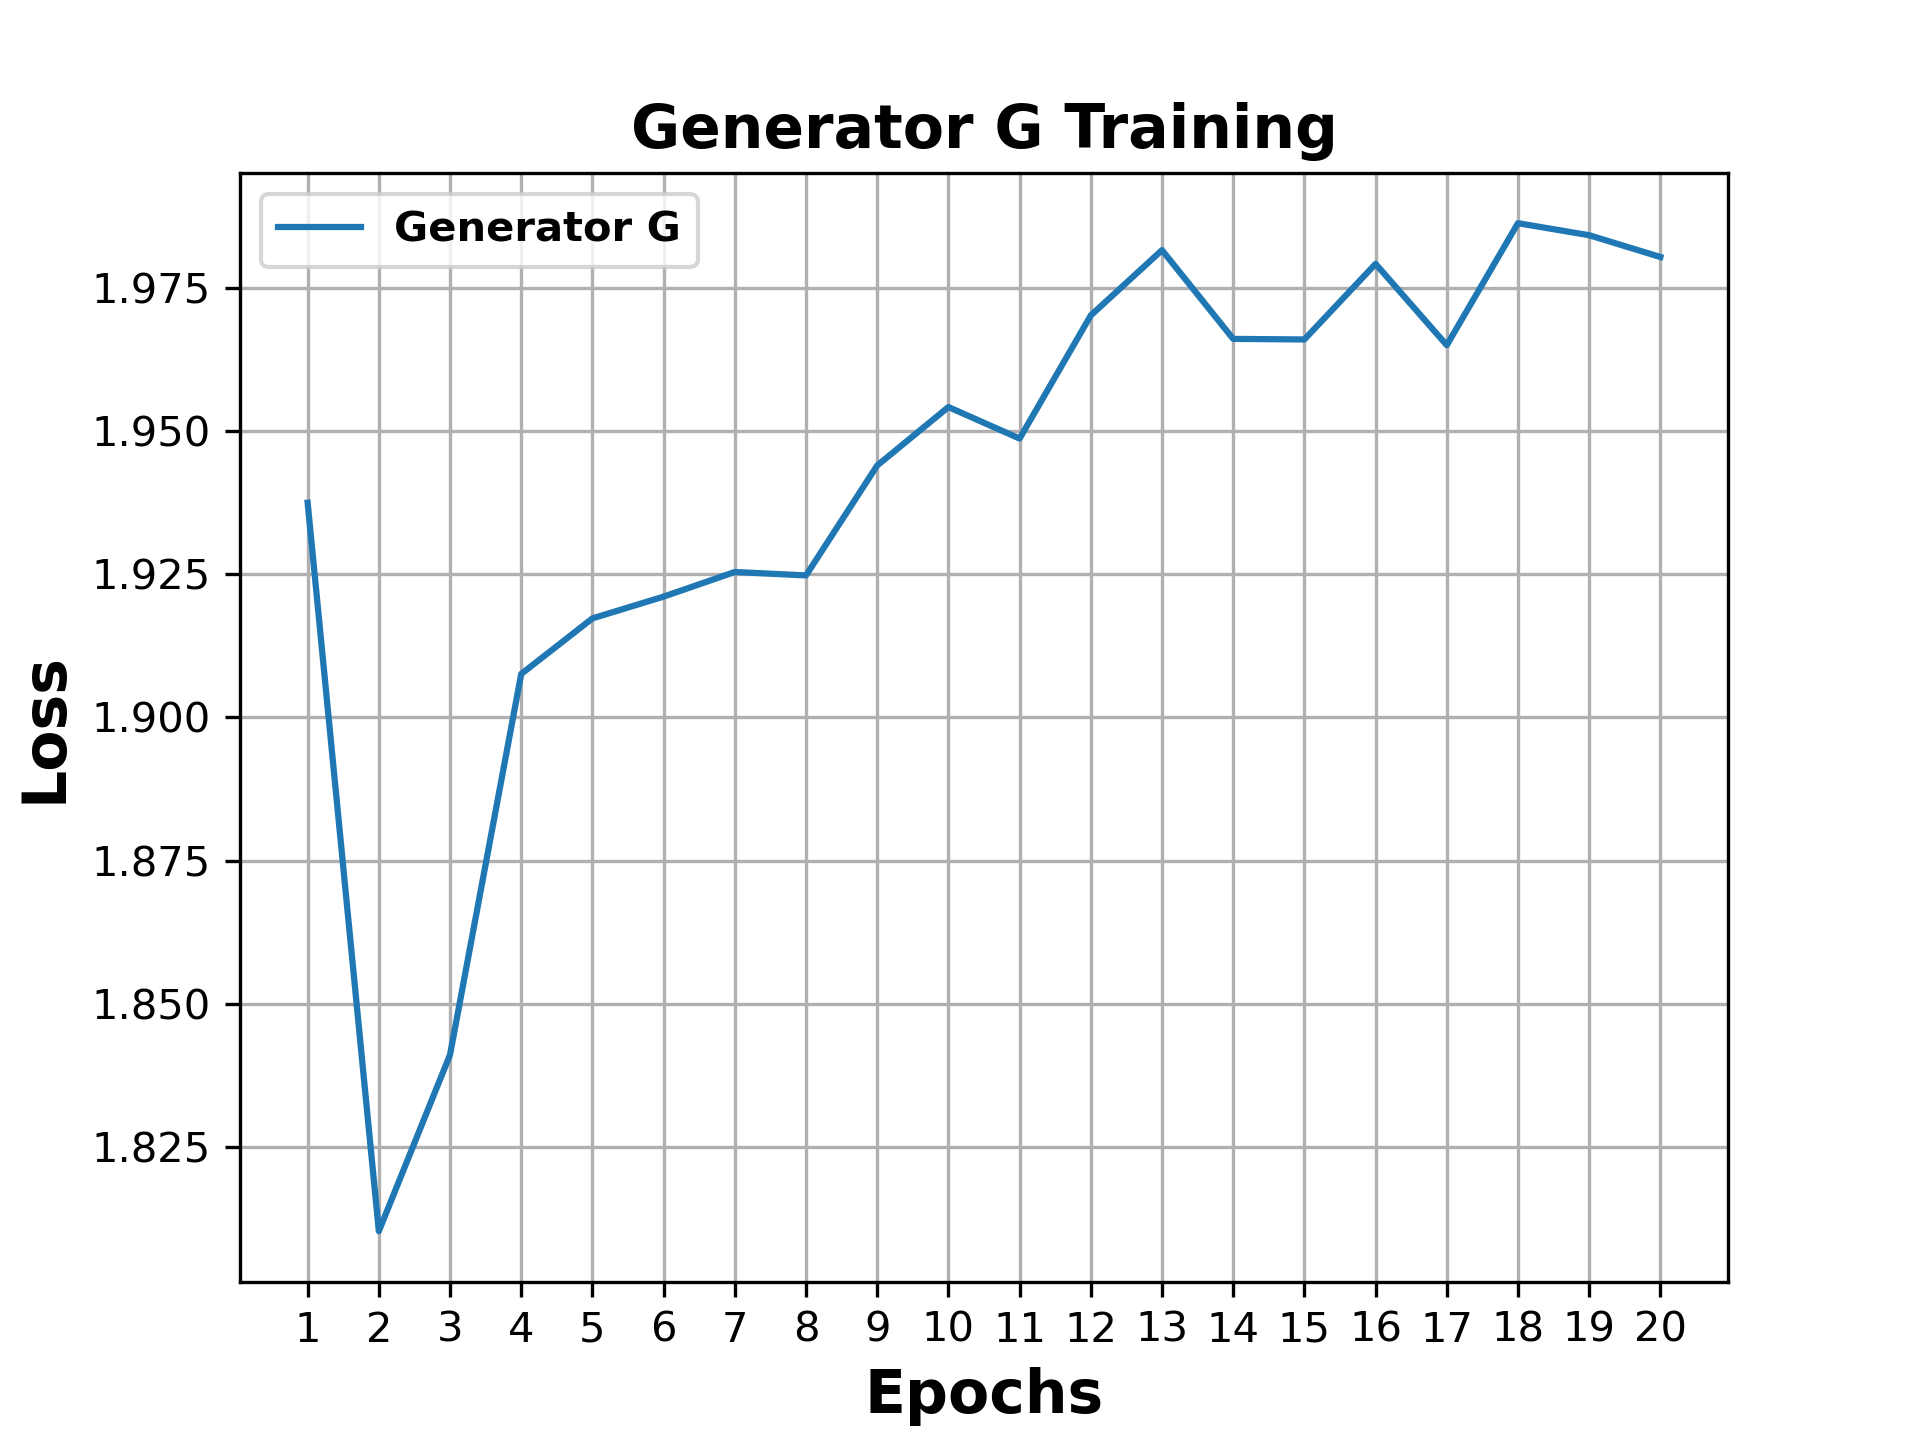
\includegraphics[width=\textwidth]{images/Evaluation/GeneratorGTraining.png}
    \caption[\ac{CycleGAN} generator $G$ training epochs vs loss plot.]{\ac{CycleGAN} generator $G$ training epochs vs loss plot.}
    \label{fig:generatorG}
  \end{minipage}
  \hfill
  \begin{minipage}[b]{0.49\textwidth}
    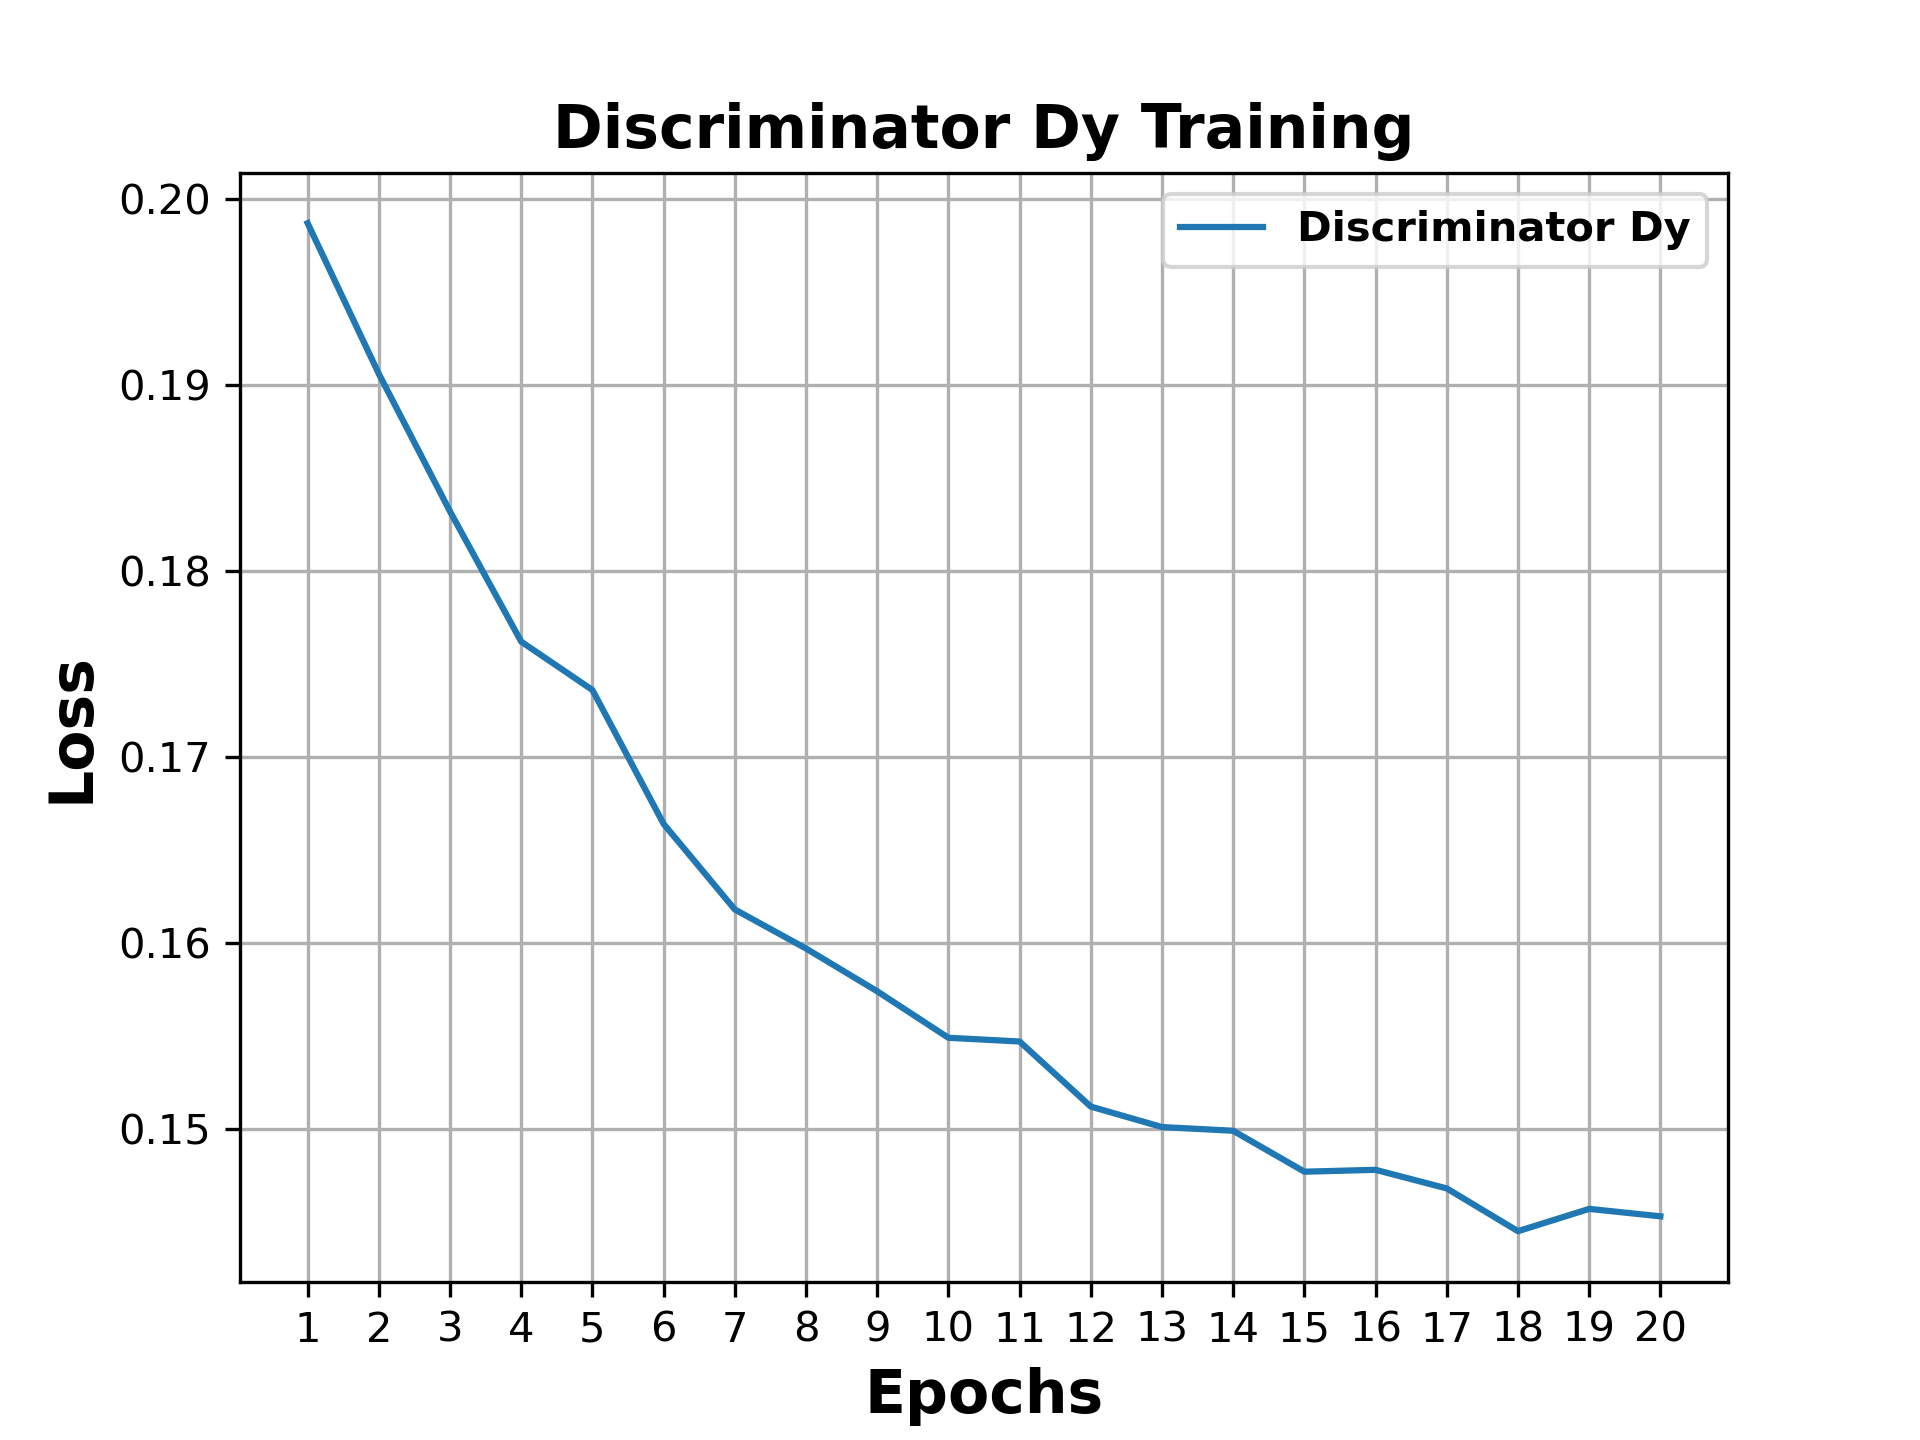
\includegraphics[width=\textwidth]{images/Evaluation/DiscriminatorDyTraining.png}
    \caption[\ac{CycleGAN} discriminator $D_Y$ training epochs vs loss plot.]{\ac{CycleGAN} discriminator $D_Y$ training epochs vs loss plot.}
    \label{fig:discriminatorDy}
  \end{minipage}
\end{figure}

\begin{figure}[H]
  \centering
  \begin{minipage}[b]{0.49\textwidth}
    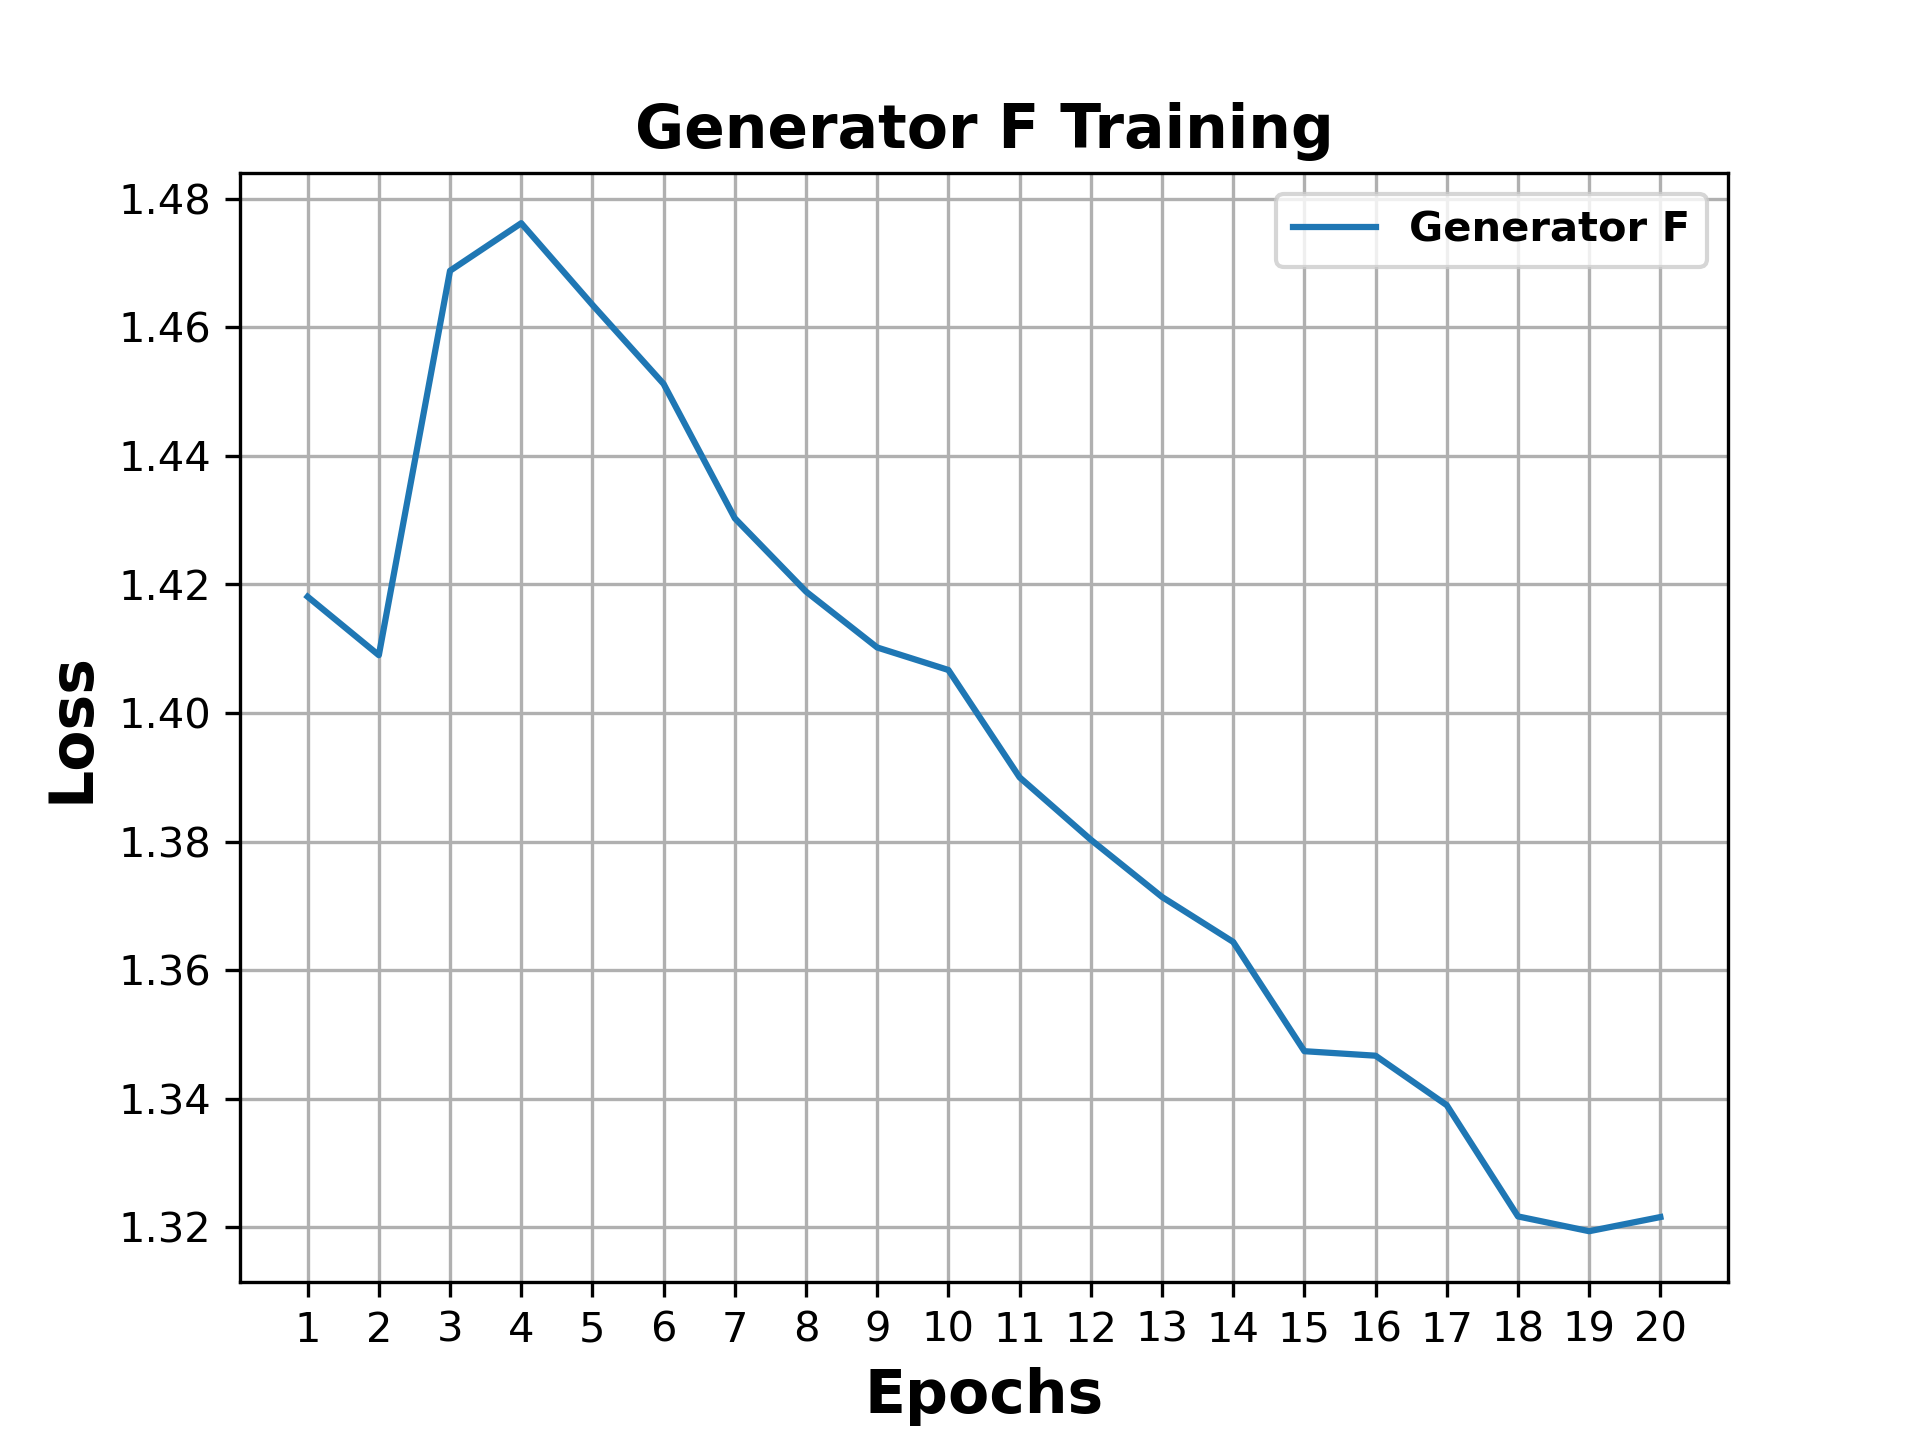
\includegraphics[width=\textwidth]{images/Evaluation/GeneratorFTraining.png}
    \caption[\ac{CycleGAN} generator $F$ training epochs vs loss plot.]{\ac{CycleGAN} generator $F$ training epochs vs loss plot.}
    \label{fig:generatorF}
  \end{minipage}
  \hfill
  \begin{minipage}[b]{0.49\textwidth}
    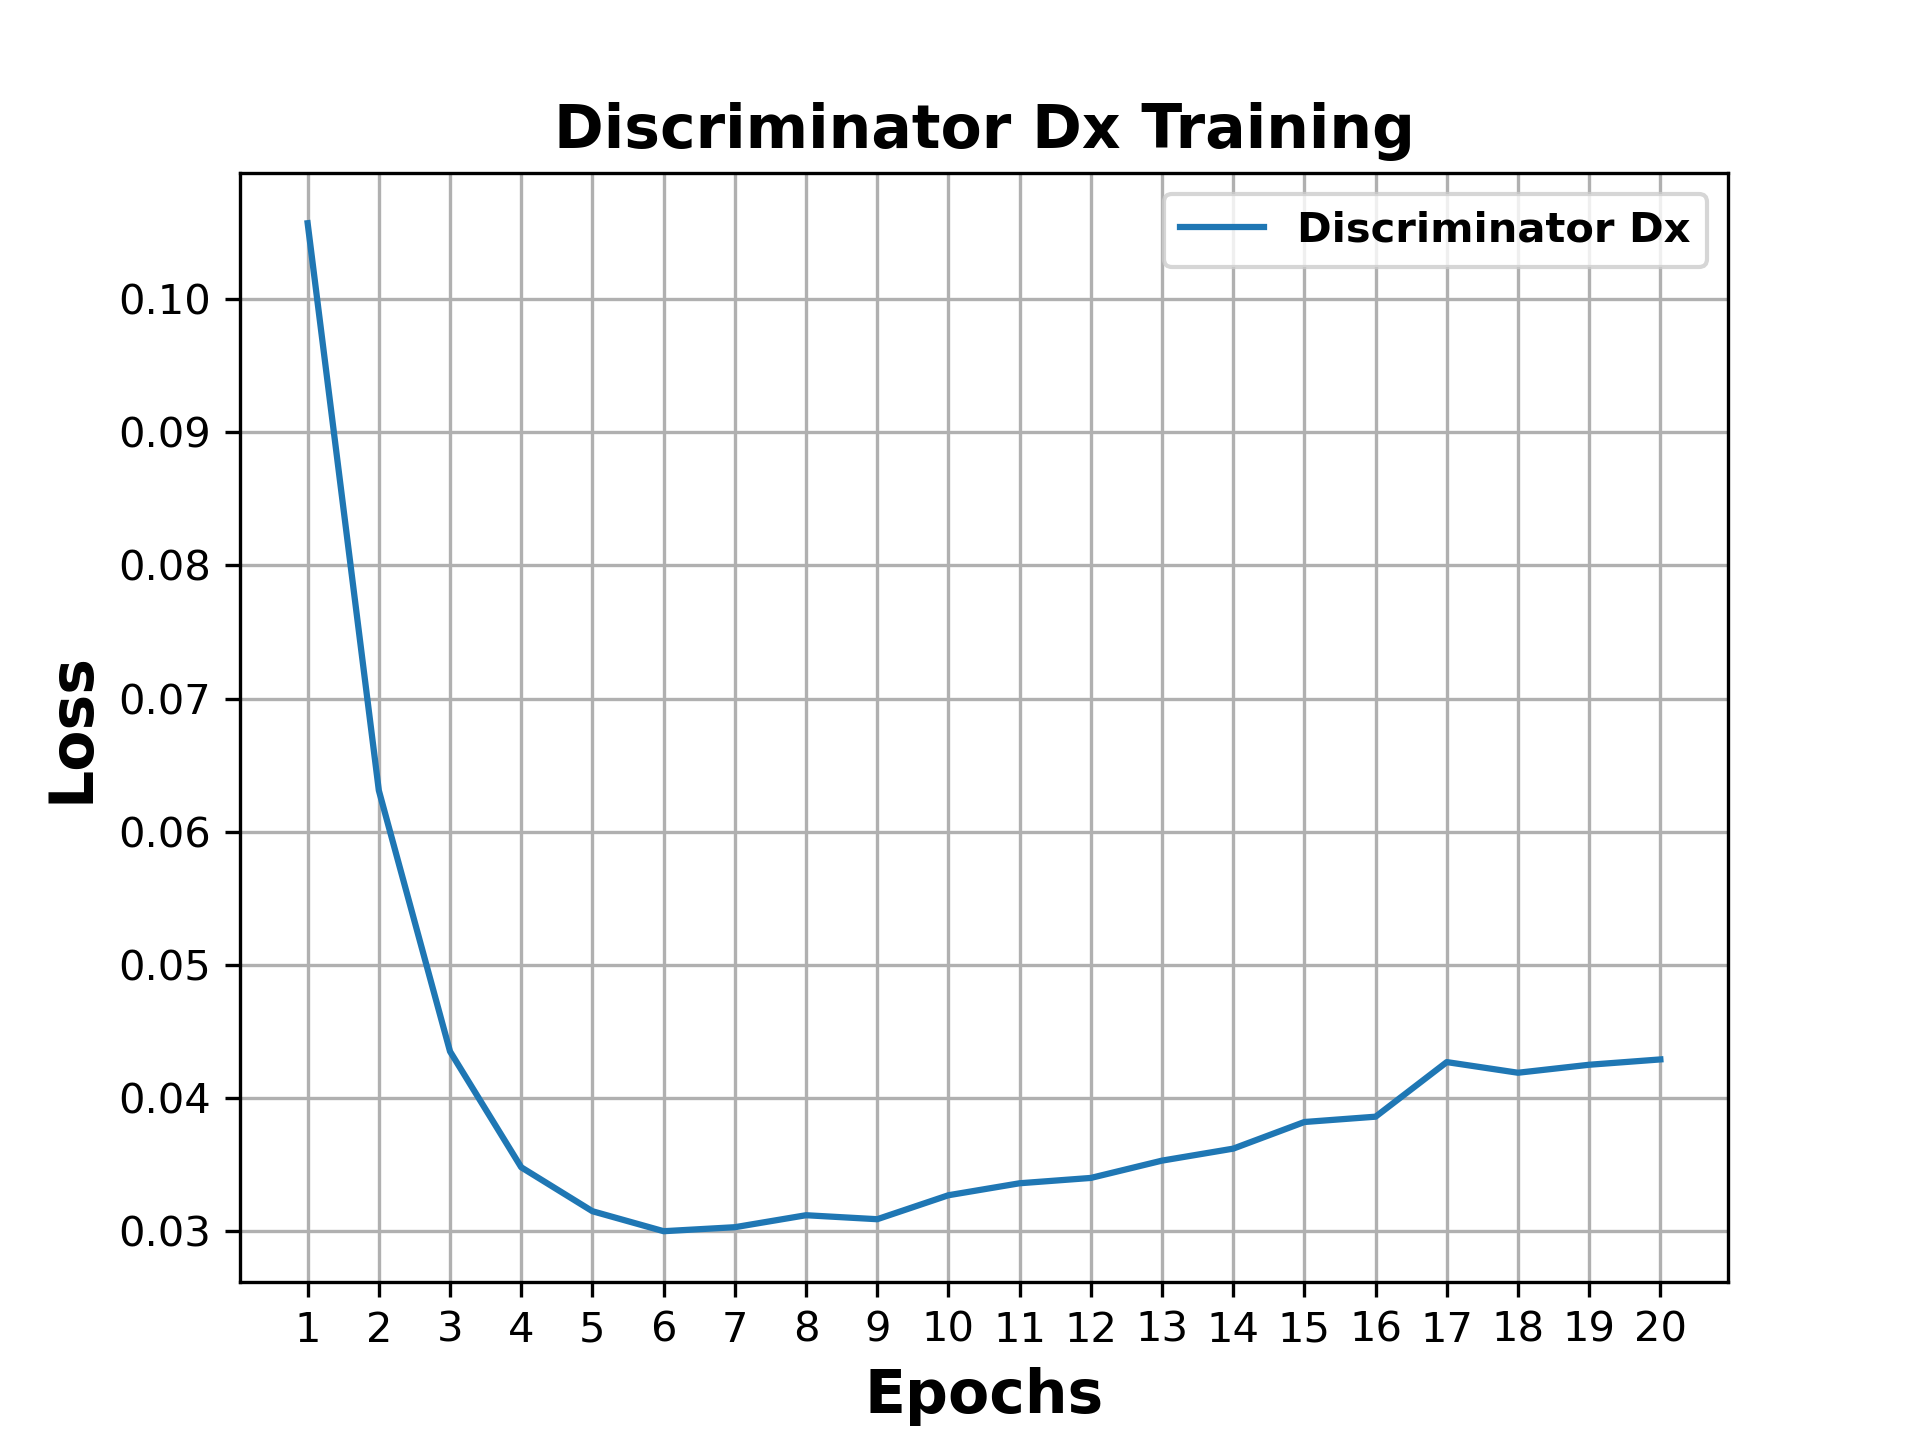
\includegraphics[width=\textwidth]{images/Evaluation/DiscriminatorDxTraining.png}
    \caption[\ac{CycleGAN} discriminator $D_X$ training epochs vs loss plot.]{\ac{CycleGAN} discriminator $D_X$ training epochs vs loss plot.}
    \label{fig:discriminatorDx}
  \end{minipage}
\end{figure}

The \ac{CycleGAN} training happens by calculating loss and updating the weights of discriminators $D_X$ and $D_Y$, and generators $G$ and $F$ respectively. First, random input images $x_i$ and $y_i$ are retrieved from source domain $X$ and target domain $Y$. The fake image generated using generator $G$ is $Generated\_Y$ and the fake image generated using generator by $F$ is $Generated\_X$. As we described earlier, $G$ is a mapping function to transform an image from source domain $X$ to target domain $Y$, mathematically it is $G: X \rightarrow Y$. And $F$ is vice versa $F: Y \rightarrow X$. The generator $G$ is called the forward generator, and $F$ is called the backward generator. First, the discriminator loss for $D_X$ and $D_Y$ on real and fake images is computed. The computed discriminator loss is used to update the weights of both discriminators. Next, cycle-consistency loss is calculated by transforming the source domain image into the target domain, back again into the source domain. It is called forward cycle-consistency loss. It is calculated by determining the difference between the original image in the source domain and cycled image back in the source domain. If you refer to figure \ref{fig:GxyFyx}, the forward cycle-consistency loss is the difference between \textit{Input\_X} and \textit{Cyclic\_X}. The backward cycle-consistency loss is calculated by transforming the target domain image into the source domain, back again into the target domain. In figure \ref{fig:GxyFyx}, the backward cycle-consistency loss is the difference between \textit{Input\_Y} and \textit{Cyclic\_Y}. The cycle-consistency loss forces generating an image that is context instead of generating random images.

Further, identity mapping loss is calculated to preserve the color of images after domain translation using generators $G$ and $F$. The generator $G$ transforms the image from domain $X$ to the domain $Y$. When the input $y_i$ is given to generator $G$ from the target domain $Y$, it should produce an identical image. The identity mapping loss for generator $G$ is the difference between the original image $y_i$, and the transformed image \textit{Same\_Y} when $y_i$ is used as an input for $G$. And, the identity mapping loss for generator $F$ is the difference between input image $x_i$ and the transformed image \textit{Same\_X} when $x_i$ is used as an input for $F$. The generator loss for generators $G$ and $F$ is calculated by the feedback given by their respective discriminators $D_Y$ and $D_X$. Combining generator loss, cycle-consistency loss, and identity mapping loss, the total generator loss is calculated separately for generators $G$ and $F$, and their weights are updated to produce quality images. The epochs against loss plot while training generators $G$ and $F$ are shown in figure \ref{fig:generatorG} and \ref{fig:generatorF} respectively. Also, the epochs against loss plot while training discriminators $D_X$ and $D_Y$ are shown in figure \ref{fig:discriminatorDx} and \ref{fig:discriminatorDy} respectively. To understand the algorithm of \ac{CycleGAN} in-depth, refer to the pseudo-code from \ref{alg:CycleGANAlgorithm}.



\subsection{Training a Classifier on Synthetic Document Images}\label{trainingsyntheticclassifier}

Before this experiment, the dataset of synthetic document images is created using templates (figure \ref{fig:template}) and handwritten crops (figure \ref{fig:keinwifi}) using the process mentioned in figure \ref{fig:InsertHandwrittenCrops}. In this experiment, a simple classifier (table \ref{table:ClassifierArchitecture}), is trained on synthetic document images dataset. The performance of this classifier is evaluated on annotated real document images (test dataset) to understand the domain gap between real data distribution and synthetic data distribution. The classification report in table \ref{table:SyntheticClassificationReport} states that the accuracy of this classifier on real document images is 25\%, macro average f1-score is 27\%, and weighted average f1-score is 31\%. As mentioned earlier, the test dataset is unbalanced, the weighted average f1-score is a suitable metric in this scenario. The weighted average f1-score concludes that there is a huge gap between real data distribution and synthetic data distribution. The confusion matrix is illustrated in figure \ref{fig:CMCycleganGeneratedDocumentImagesClassifier}. Where it is completely visible most of the test images were classified wrongly. The epochs against accuracy and epochs against loss plots while training classifier on synthetic document images is illustrated in figure \ref{fig:SyntheticClassifierAcc} and \ref{fig:SyntheticClassifierLoss} respectively.

\begin{figure}[H]
  \centering
  \begin{minipage}[b]{0.49\textwidth}
    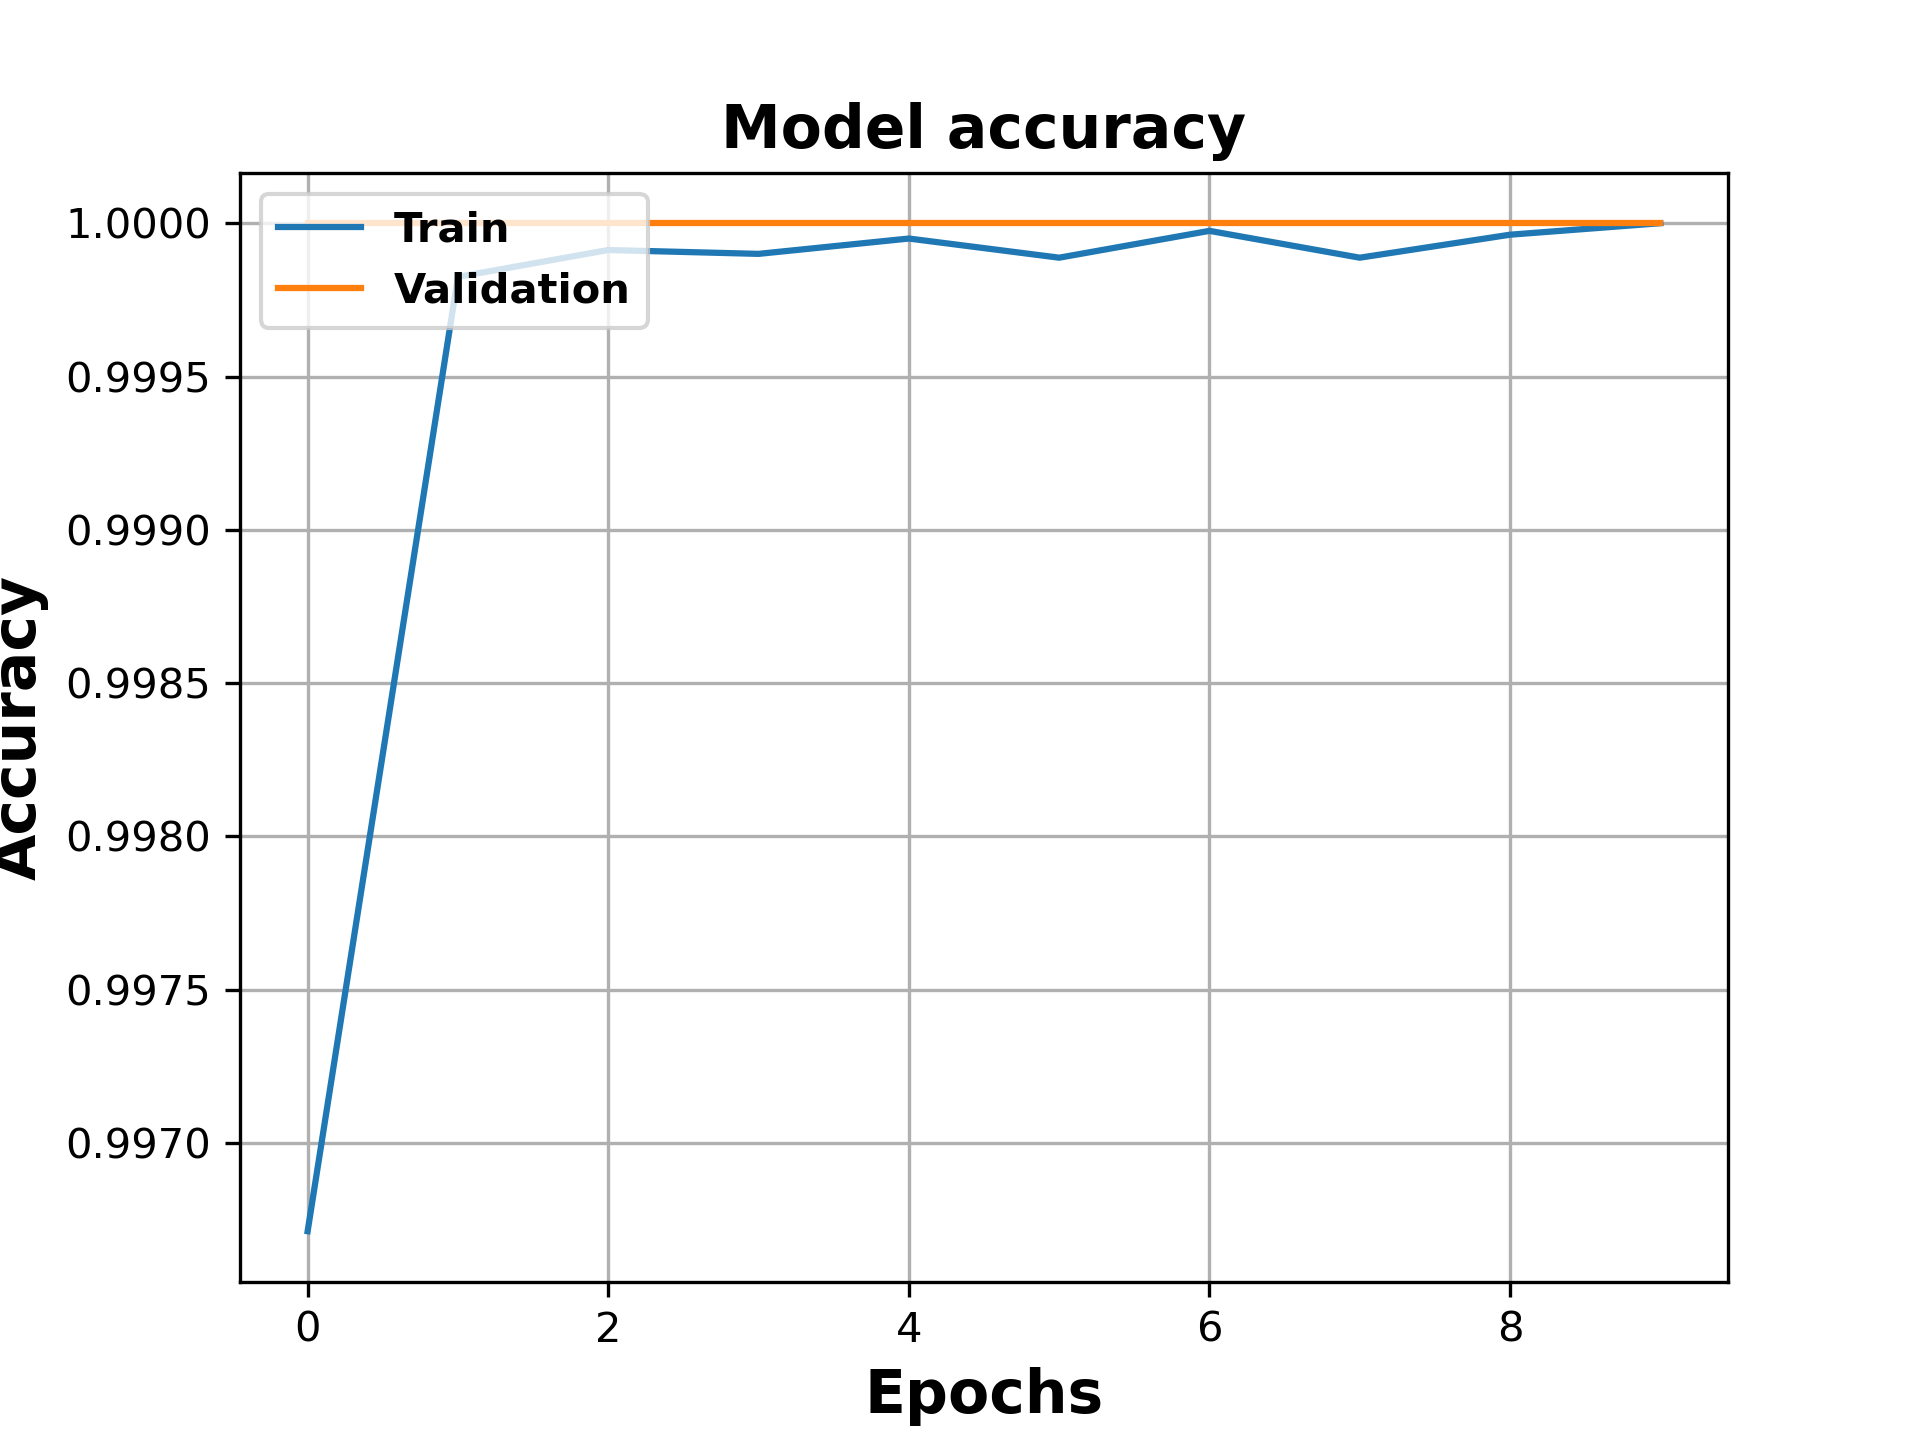
\includegraphics[width=\textwidth]{images/Evaluation/Synthetic_Data_Classifier_2021-05-31_16-40-33_Accuracy.png}
    \caption[Epochs vs accuracy plot while training a classifier on synthetic document images.]{Epochs vs accuracy plot while training a classifier on synthetic document images.}
    \label{fig:SyntheticClassifierAcc}
  \end{minipage}
  \hfill
  \begin{minipage}[b]{0.49\textwidth}
    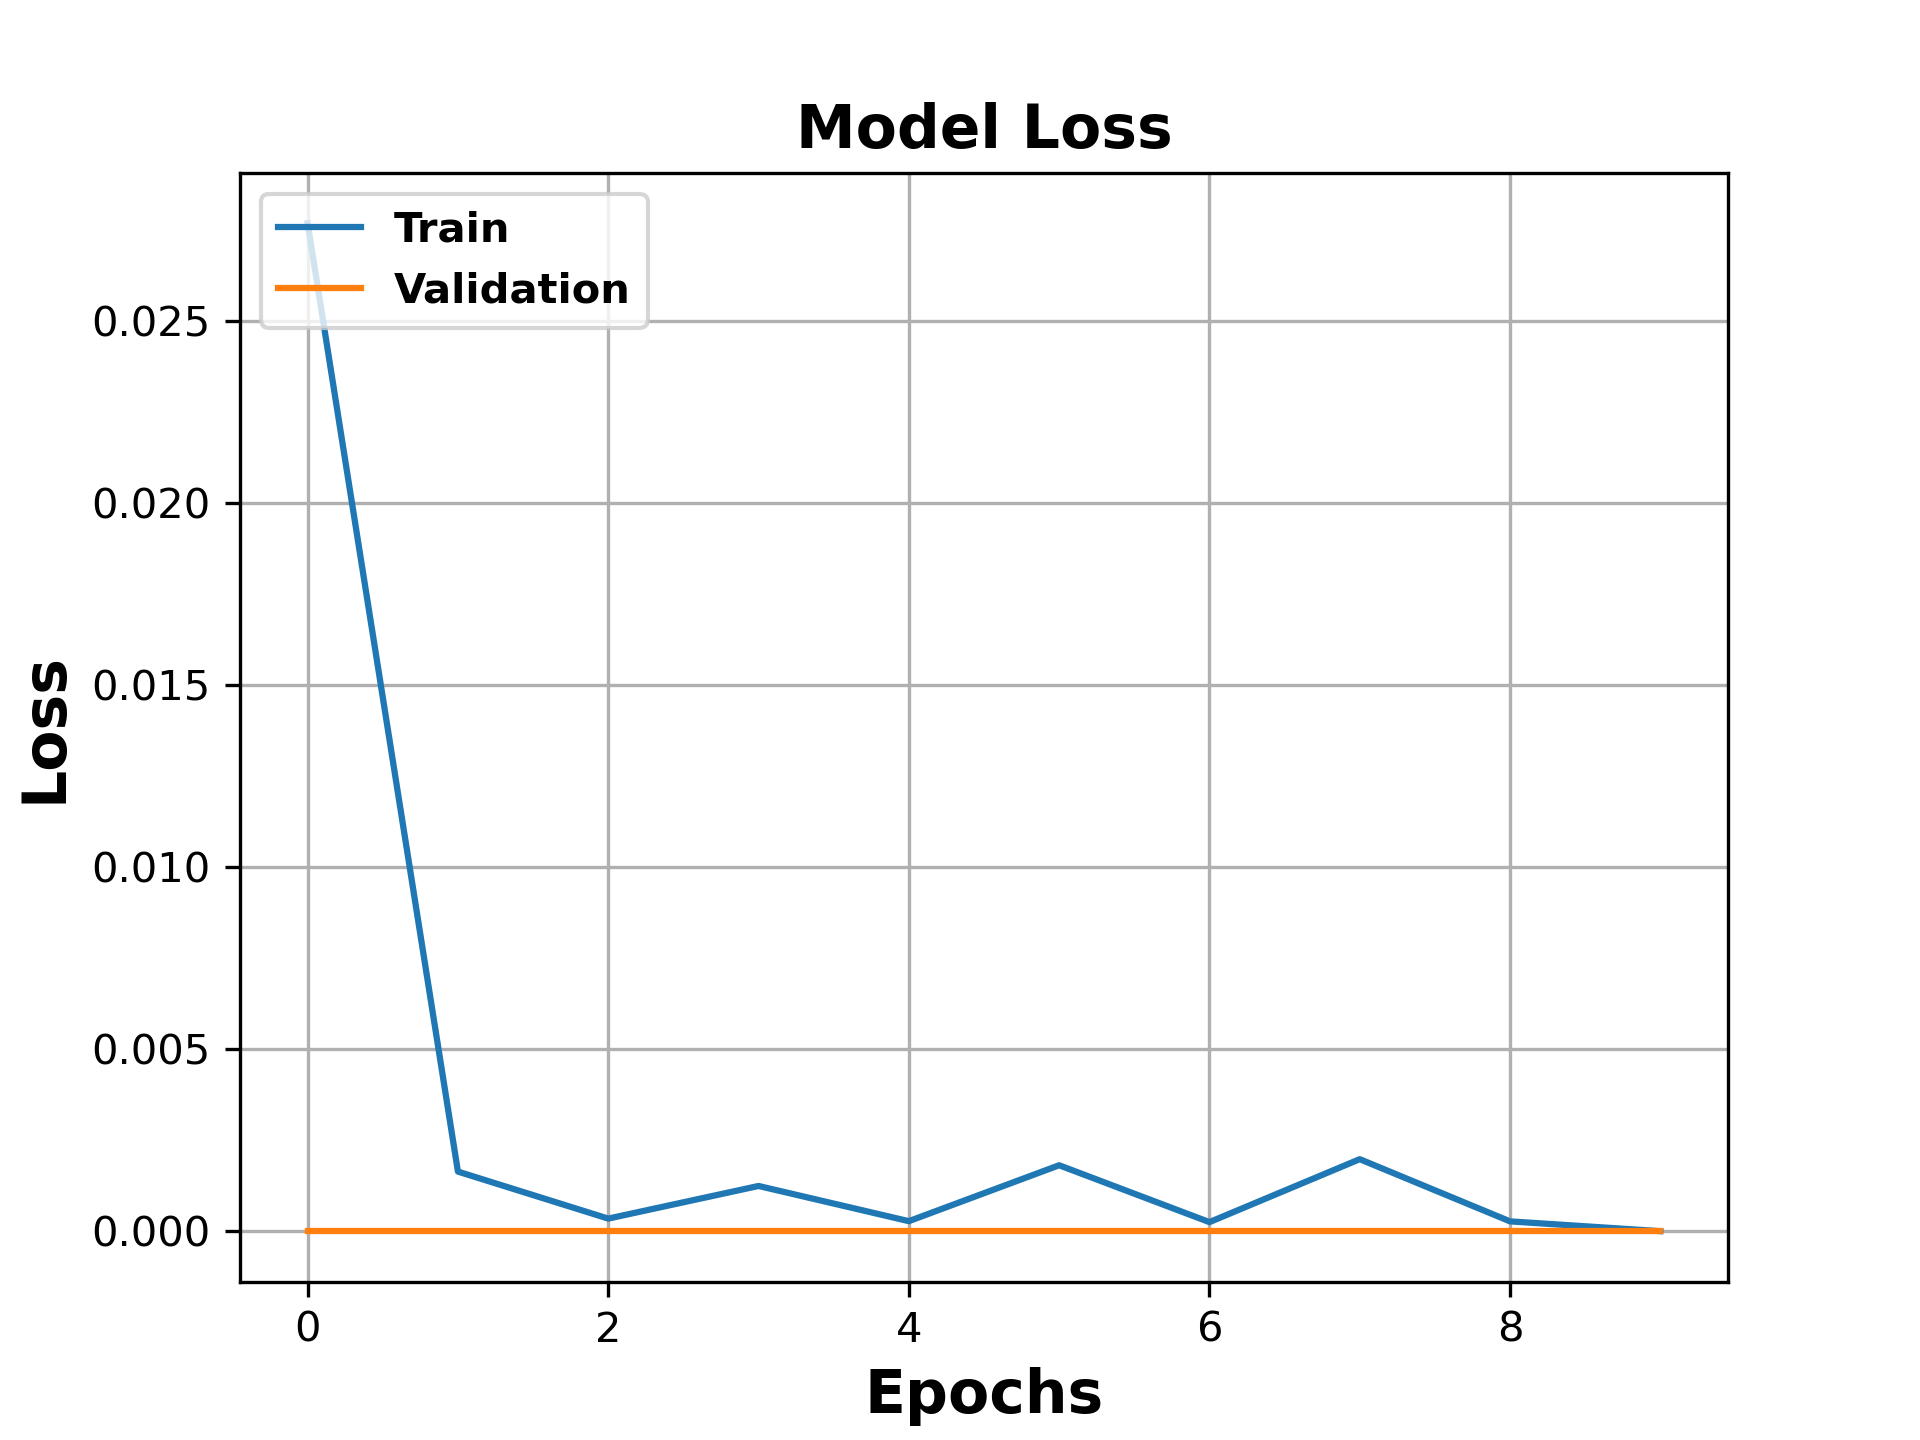
\includegraphics[width=\textwidth]{images/Evaluation/Synthetic_Data_Classifier_2021-05-31_16-40-33_Loss.png}
    \caption[Epochs vs loss plot while training a classifier on synthetic document images.]{Epochs vs loss plot while training a classifier on synthetic document images.}
    \label{fig:SyntheticClassifierLoss}
  \end{minipage}
\end{figure}


\begin{center}
\begin{table}[H]
    \centering
    \begin{center}
    \begin{tabular}{P{0.22\linewidth} P{0.10\linewidth} P{0.10\linewidth} P{0.10\linewidth} P{0.10\linewidth}} 
        \toprule
            & Precision & Recall & f1-score & Support\\[0.0ex] 
        \midrule
        DE\_LY\_Arm\_2020-01 & 0.65 & 0.50 & 0.56 & 44\\[0.0ex]
        \midrule
        DE\_LY\_Bein\_2018-08 & 0.50 & 0.02 & 0.04 & 47\\[0.0ex]
        \midrule
        DE\_LY\_Bein\_2019-01 & 0.06 & 0.90 & 0.11 & 50\\[0.0ex]
        \midrule
        DE\_LY\_Bein\_2019-07 & 0.36 & 0.20 & 0.26 & 60\\[0.0ex]
        \midrule
        DE\_LY\_Bein\_2020-01 & 0.96 & 0.21 & 0.34 & 624\\[0.0ex]
        \midrule
        DE\_LY\_Bein\_2020-03 & 0.24 & 0.25 & 0.24 & 128\\[0.0ex]
        \midrule
        DE\_LY\_Hand\_2020-01 & 0.70 & 0.44 & 0.54 & 16\\[0.0ex]
        \midrule
        DE\_PH\_Bein\_2018-09 & 0.10 & 0.14 & 0.12 & 22\\[0.0ex]
        \midrule
        DE\_PH\_Bein\_2019-02 & 0.12 & 0.04 & 0.06 & 28\\[0.0ex]
        \midrule
        DE\_PH\_Bein\_2020-01 & 0.95 & 0.51 & 0.26 & 143\\[0.0ex]
        \midrule
        \midrule
        Accuracy              &      &      & \bf{0.25} & 1162\\[0.0ex]
        Macro average             & 0.46 & 0.29 &  \bf{0.27} & 1162\\[0.0ex]
        Weighted average          & 0.74 & 0.25 &  \bf{0.31} & 1162\\[0.0ex]
        \bottomrule
    \end{tabular}
    \caption[Classification report generated after the classifier is trained on synthetic document images, its classification performance evaluated on the annotated real document images.]{Classification report generated after the classifier is trained on synthetic document images, its classification performance evaluated on the annotated real document images.}
    \label{table:SyntheticClassificationReport}
    \end{center}
\end{table}
\end{center}



\subsection{Training a Classifier on \ac{CycleGAN} Generated Document Images}\label{trainingCycleGANDataClassifier}


This is the most important experiment of this thesis. After the \ac{CycleGAN} is trained, the generator $G$ is loaded from the saved checkpoint, to perform image-to-image translation, simply to say, transforming synthetic document images to realistic document images. 100,000 synthetic document images are transformed into realistic document images. The transformed 100,000 realistic document images are used to train the same classifier (table \ref{table:ClassifierArchitecture}). The performance of this classifier is evaluated on annotated real document images (test dataset) to understand the domain gap between real data distribution and \ac{CycleGAN} generated data distribution and quality of generated images compared to real images. The classification report in table \ref{table:CycleGANClassificationReport} states that the accuracy of this classifier on annotated real document images is 27\%, macro average f1-score is 34\%, and weighted average f1-score is 25\%. The majority of documents are of the type ``Bein'', and they are similar to each other. It has been found, a small artifact transformation failure has caused the wrong classification because learning such minor differences and features present in training datasets by \ac{CycleGAN} was very challenging. The confusion matrix is illustrated in figure \ref{fig:CMFaxifiedDocumentImagesClassifier}. In the confusion matrix, the document images DE\_LY\_Arm\_2020-01, DE\_LY\_Bein\_2019-07,  DE\_LY\_Hand\_2020-01, and DE\_PH\_Bein\_2020-01 are classified satisfactorily. Document images DE\_LY\_Bein\_2020-01 and DE\_LY\_Bein\_2020-03 are wrongly classified as DE\_LY\_Bein\_2019-07. Document images DE\_PH\_Bein\_2018-09 and DE\_PH\_Bein\_2019-02 are wrongly classified as DE\_PH\_Bein\_2019-02. In section \ref{QualitativeResults}, qualitative results of the image-to-image translation are illustrated along with failure cases. The epochs against accuracy and epochs against loss plots while training classifier on \ac{CycleGAN} generated document images is illustrated in figure \ref{fig:CycleGANClassifierAcc} and \ref{fig:CycleGANClassifierLoss} respectively.


\begin{figure}[H]
  \centering
  \begin{minipage}[b]{0.45\textwidth}
    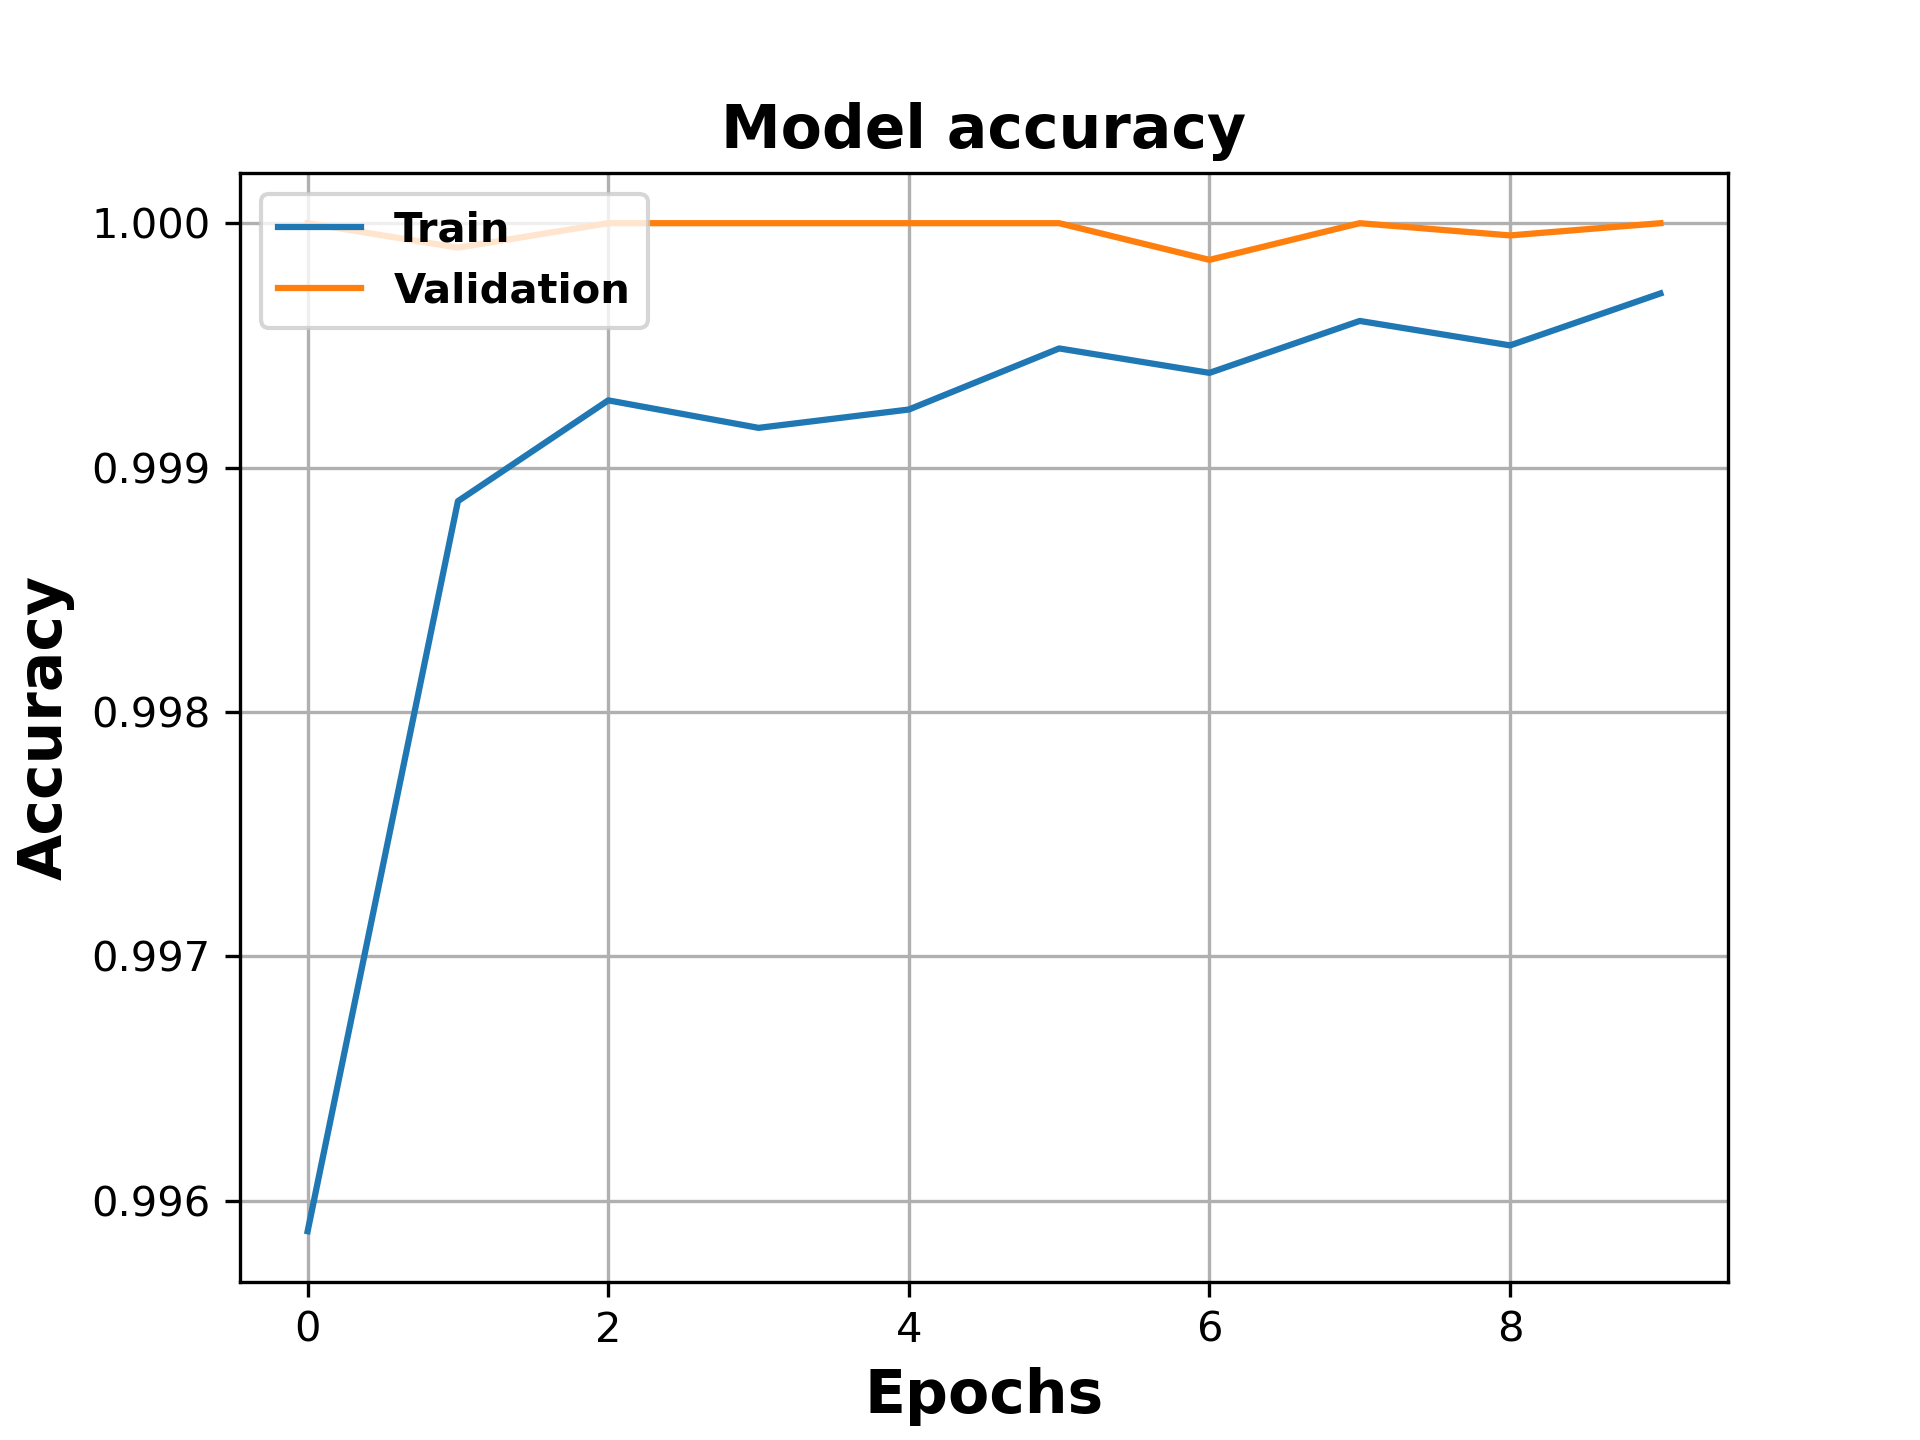
\includegraphics[width=\textwidth]{images/Evaluation/CycleGAN_Generated_Data_Classifier_2021-06-02_21-55-39_Accuracy.png}
    \caption[Epochs vs accuracy plot while training a classifier on \ac{CycleGAN} generated document images.]{Epochs vs accuracy plot while training a classifier  on \ac{CycleGAN} generated document images.}
    \label{fig:CycleGANClassifierAcc}
  \end{minipage}
  \hfill
  \begin{minipage}[b]{0.45\textwidth}
    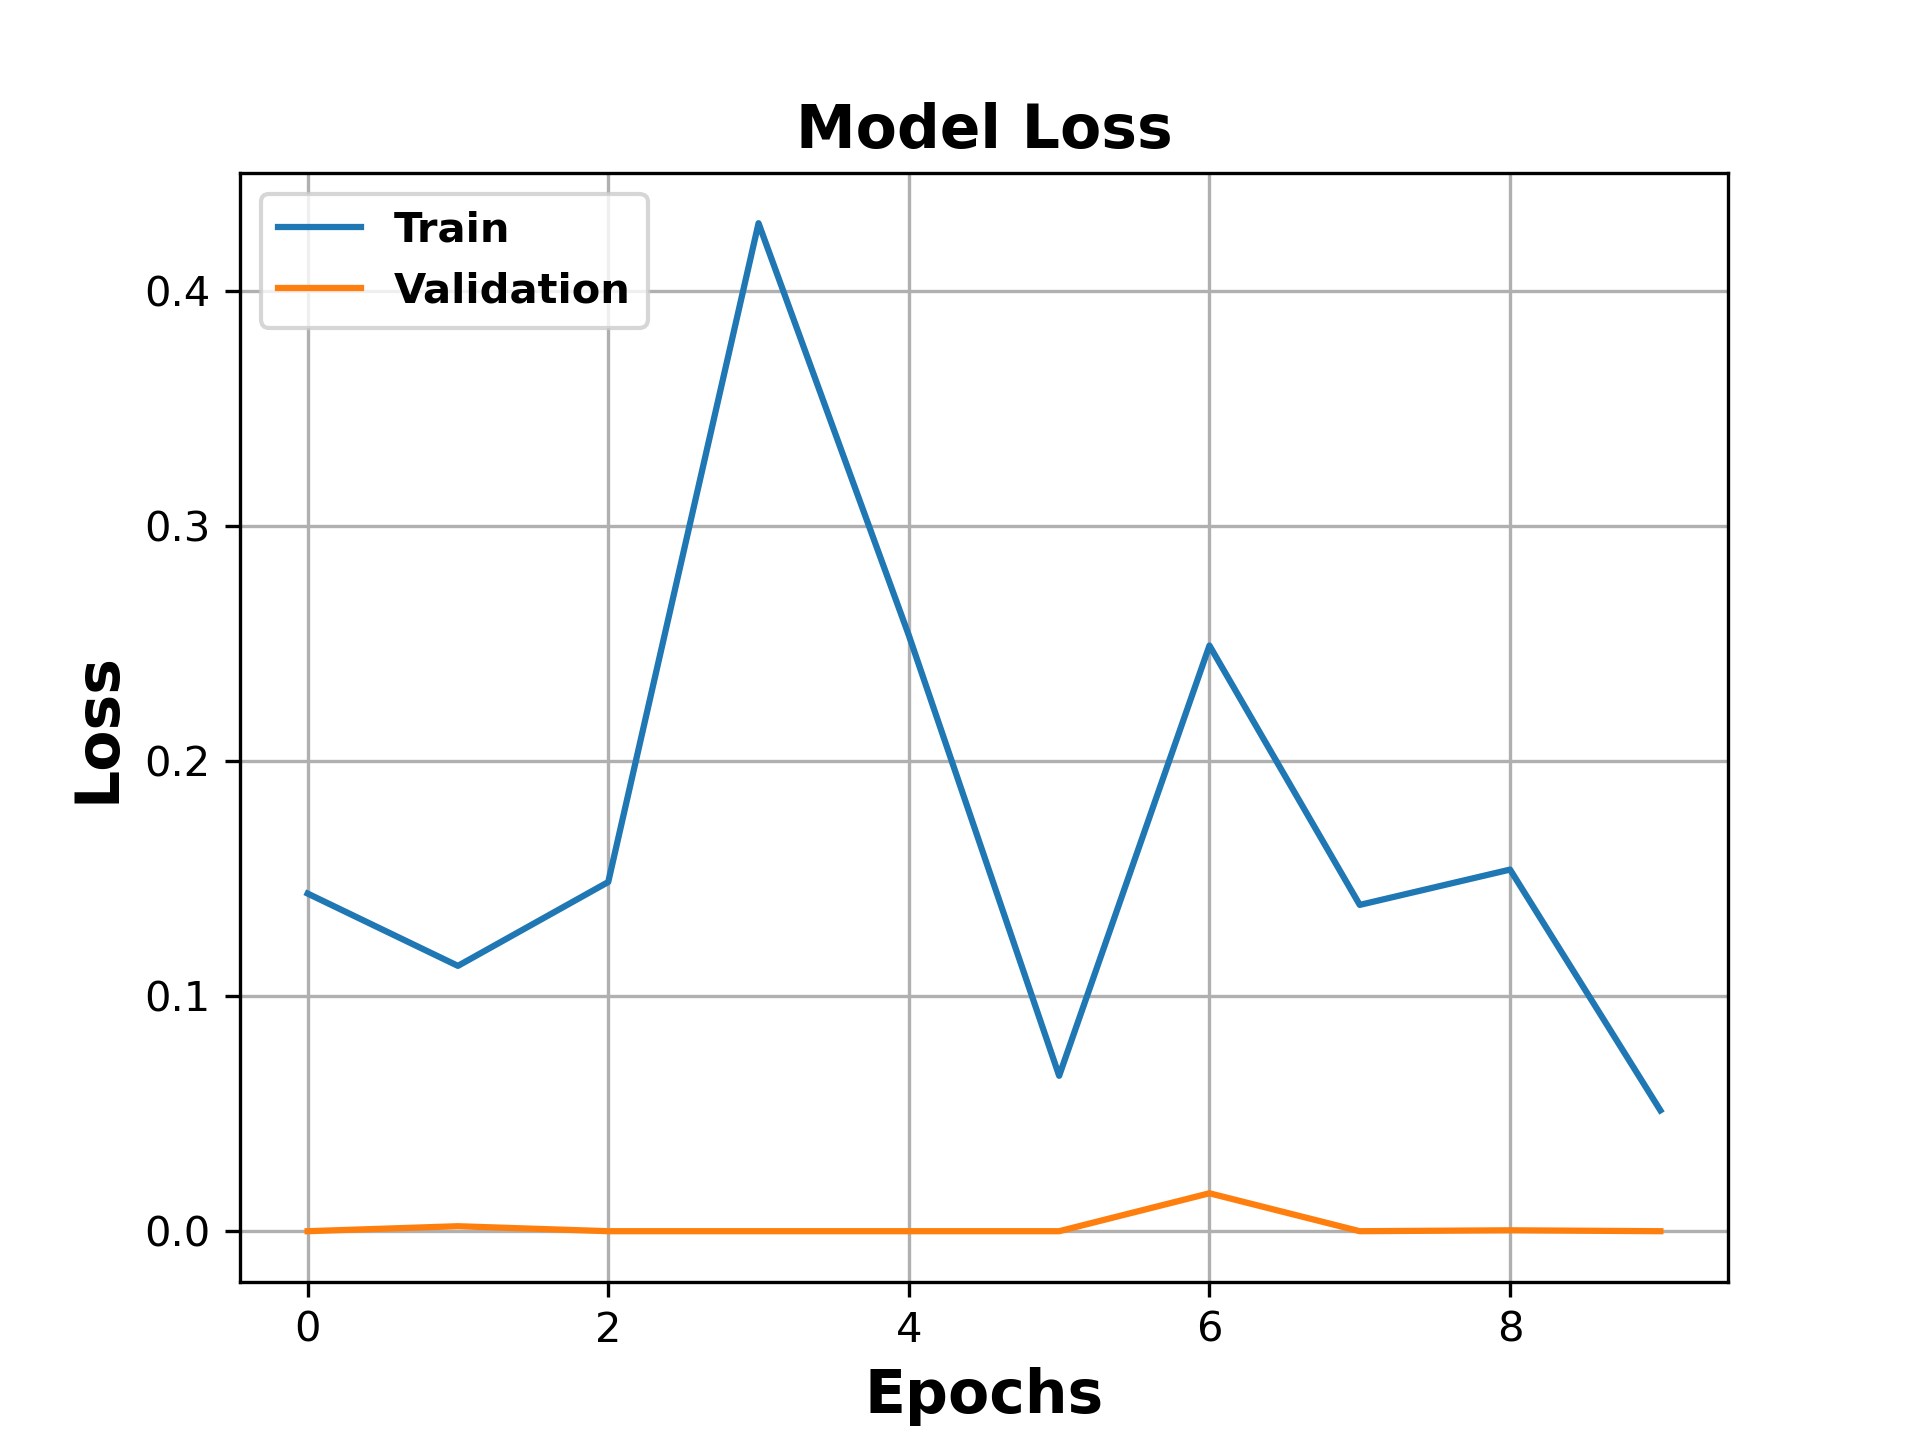
\includegraphics[width=\textwidth]{images/Evaluation/CycleGAN_Generated_Data_Classifier_2021-06-02_21-55-39_Loss.png}
    \caption[Epochs vs loss plot while training a classifier on \ac{CycleGAN} generated document images.]{Epochs vs loss plot while training a classifier on \ac{CycleGAN} generated document images.}
    \label{fig:CycleGANClassifierLoss}
  \end{minipage}
\end{figure}


\begin{center}
\begin{table}[H]
    \begin{center}
    \begin{tabular}{P{0.22\linewidth} P{0.10\linewidth} P{0.10\linewidth} P{0.10\linewidth} P{0.10\linewidth}} 
	        \toprule
            & Precision & Recall & f1-score & Support\\[0.0ex] 
        \midrule
        DE\_LY\_Arm\_2020-01 & 0.53 & 0.75 & 0.62 & 44\\[0.0ex]
        \midrule
        DE\_LY\_Bein\_2018-08 & 0.21 & 0.28 & 0.24 & 47\\[0.0ex]
        \midrule
        DE\_LY\_Bein\_2019-01 & 0.16 & 0.14 & 0.15 & 50\\[0.0ex]
        \midrule
        DE\_LY\_Bein\_2019-07 & 0.11 & 0.83 & 0.19 & 60\\[0.0ex]
        \midrule
        DE\_LY\_Bein\_2020-01 & 0.72 & 0.07 & 0.12 & 624\\[0.0ex]
        \midrule
        DE\_LY\_Bein\_2020-03 & 0.16 & 0.34 & 0.22 & 128\\[0.0ex]
        \midrule
        DE\_LY\_Hand\_2020-01 & 0.80 & 0.75 & 0.77 & 16\\[0.0ex]
        \midrule
        DE\_PH\_Bein\_2018-09 & 0.07 & 0.05 & 0.06 & 22\\[0.0ex]
        \midrule
        DE\_PH\_Bein\_2019-02 & 0.33 & 0.46 & 0.39 & 28\\[0.0ex]
        \midrule
        DE\_PH\_Bein\_2020-01 & 0.70 & 0.67 & 0.68 & 143\\[0.0ex]
        \midrule
        \midrule
        Accuracy              &      &      & \bf{0.27} & 1162\\[0.0ex]
        Macro average             & 0.38 & 0.43 &  \bf{0.34} & 1162\\[0.0ex]
        Weighted average          & 0.55 & 0.27 &  \bf{0.25} & 1162\\[0.0ex]
        \bottomrule
    \end{tabular}
    \caption[Classification report generated after the classifier is trained on \ac{CycleGAN} generated document images, its classification performance evaluated on the annotated real document images.]{Classification report generated after the classifier is trained on \ac{CycleGAN} generated document images, its classification performance evaluated on the annotated real document images.}
    \label{table:CycleGANClassificationReport}
    \end{center}
\end{table}
\end{center}




\subsection{Training a Classifier on Faxified Document Images}\label{trainingfaxifiedclassifier}


\begin{figure}[H]
        \begin{center}
	    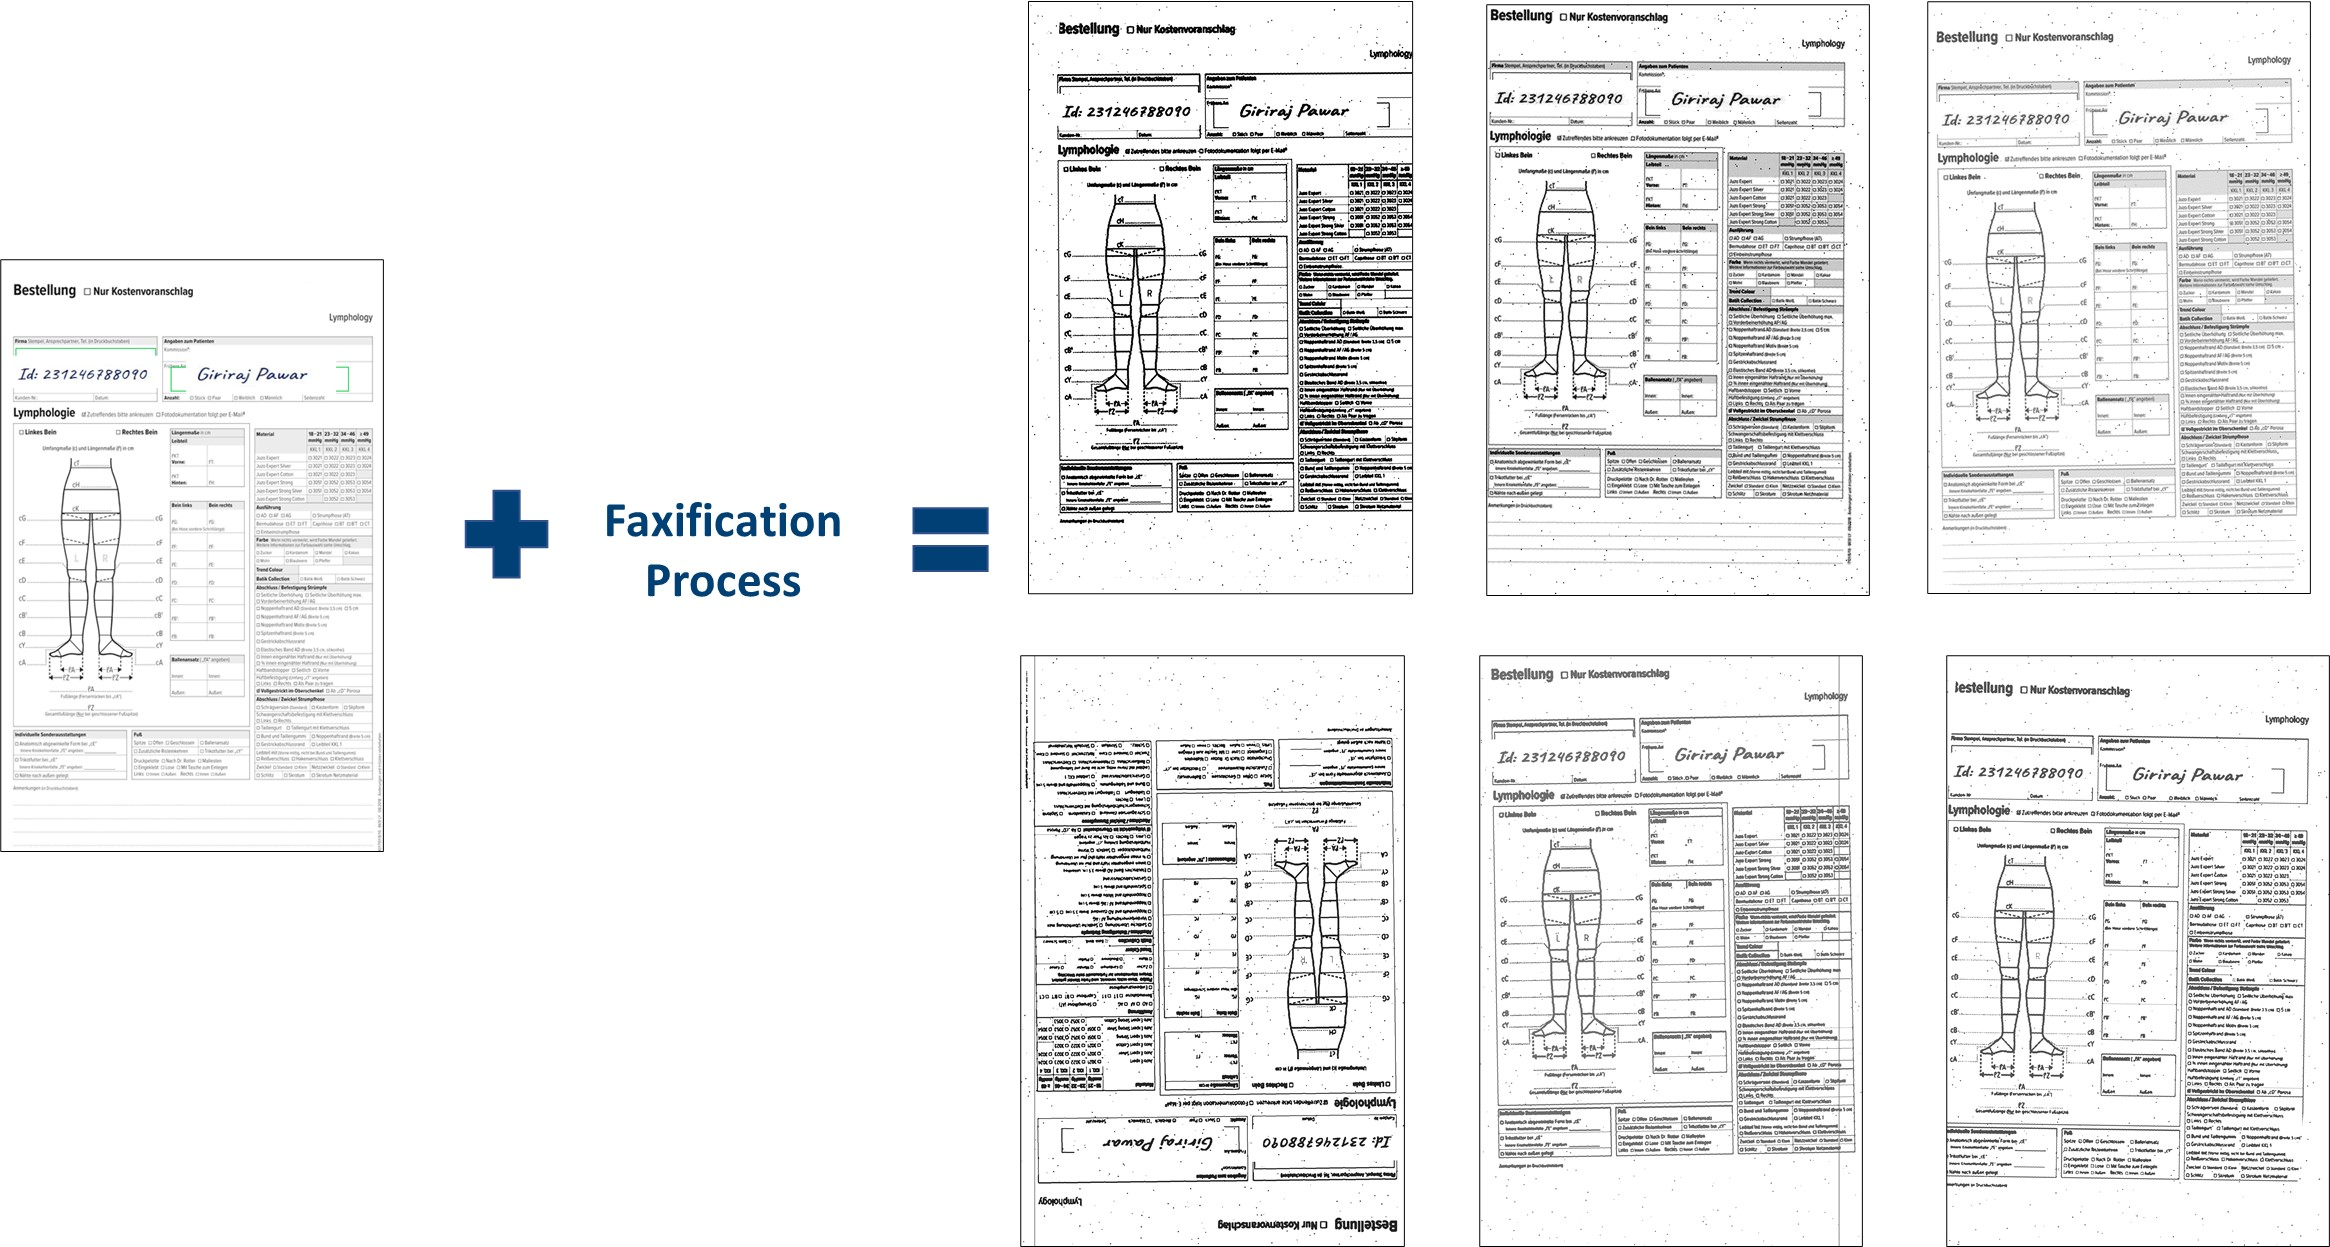
\includegraphics[scale=0.25]{images/Evaluation/FaxificationProcess.jpg}
	    \caption[Illustration of faxification process applied on synthetic document images.]{Illustration of faxification process applied on synthetic document images (figure reproduced from elevait GmbH \& Co. KG with permission).}
	    \label{fig:FaxificationProcess}
	    \end{center}
\end{figure}

\begin{figure}[H]
        \begin{center}
	    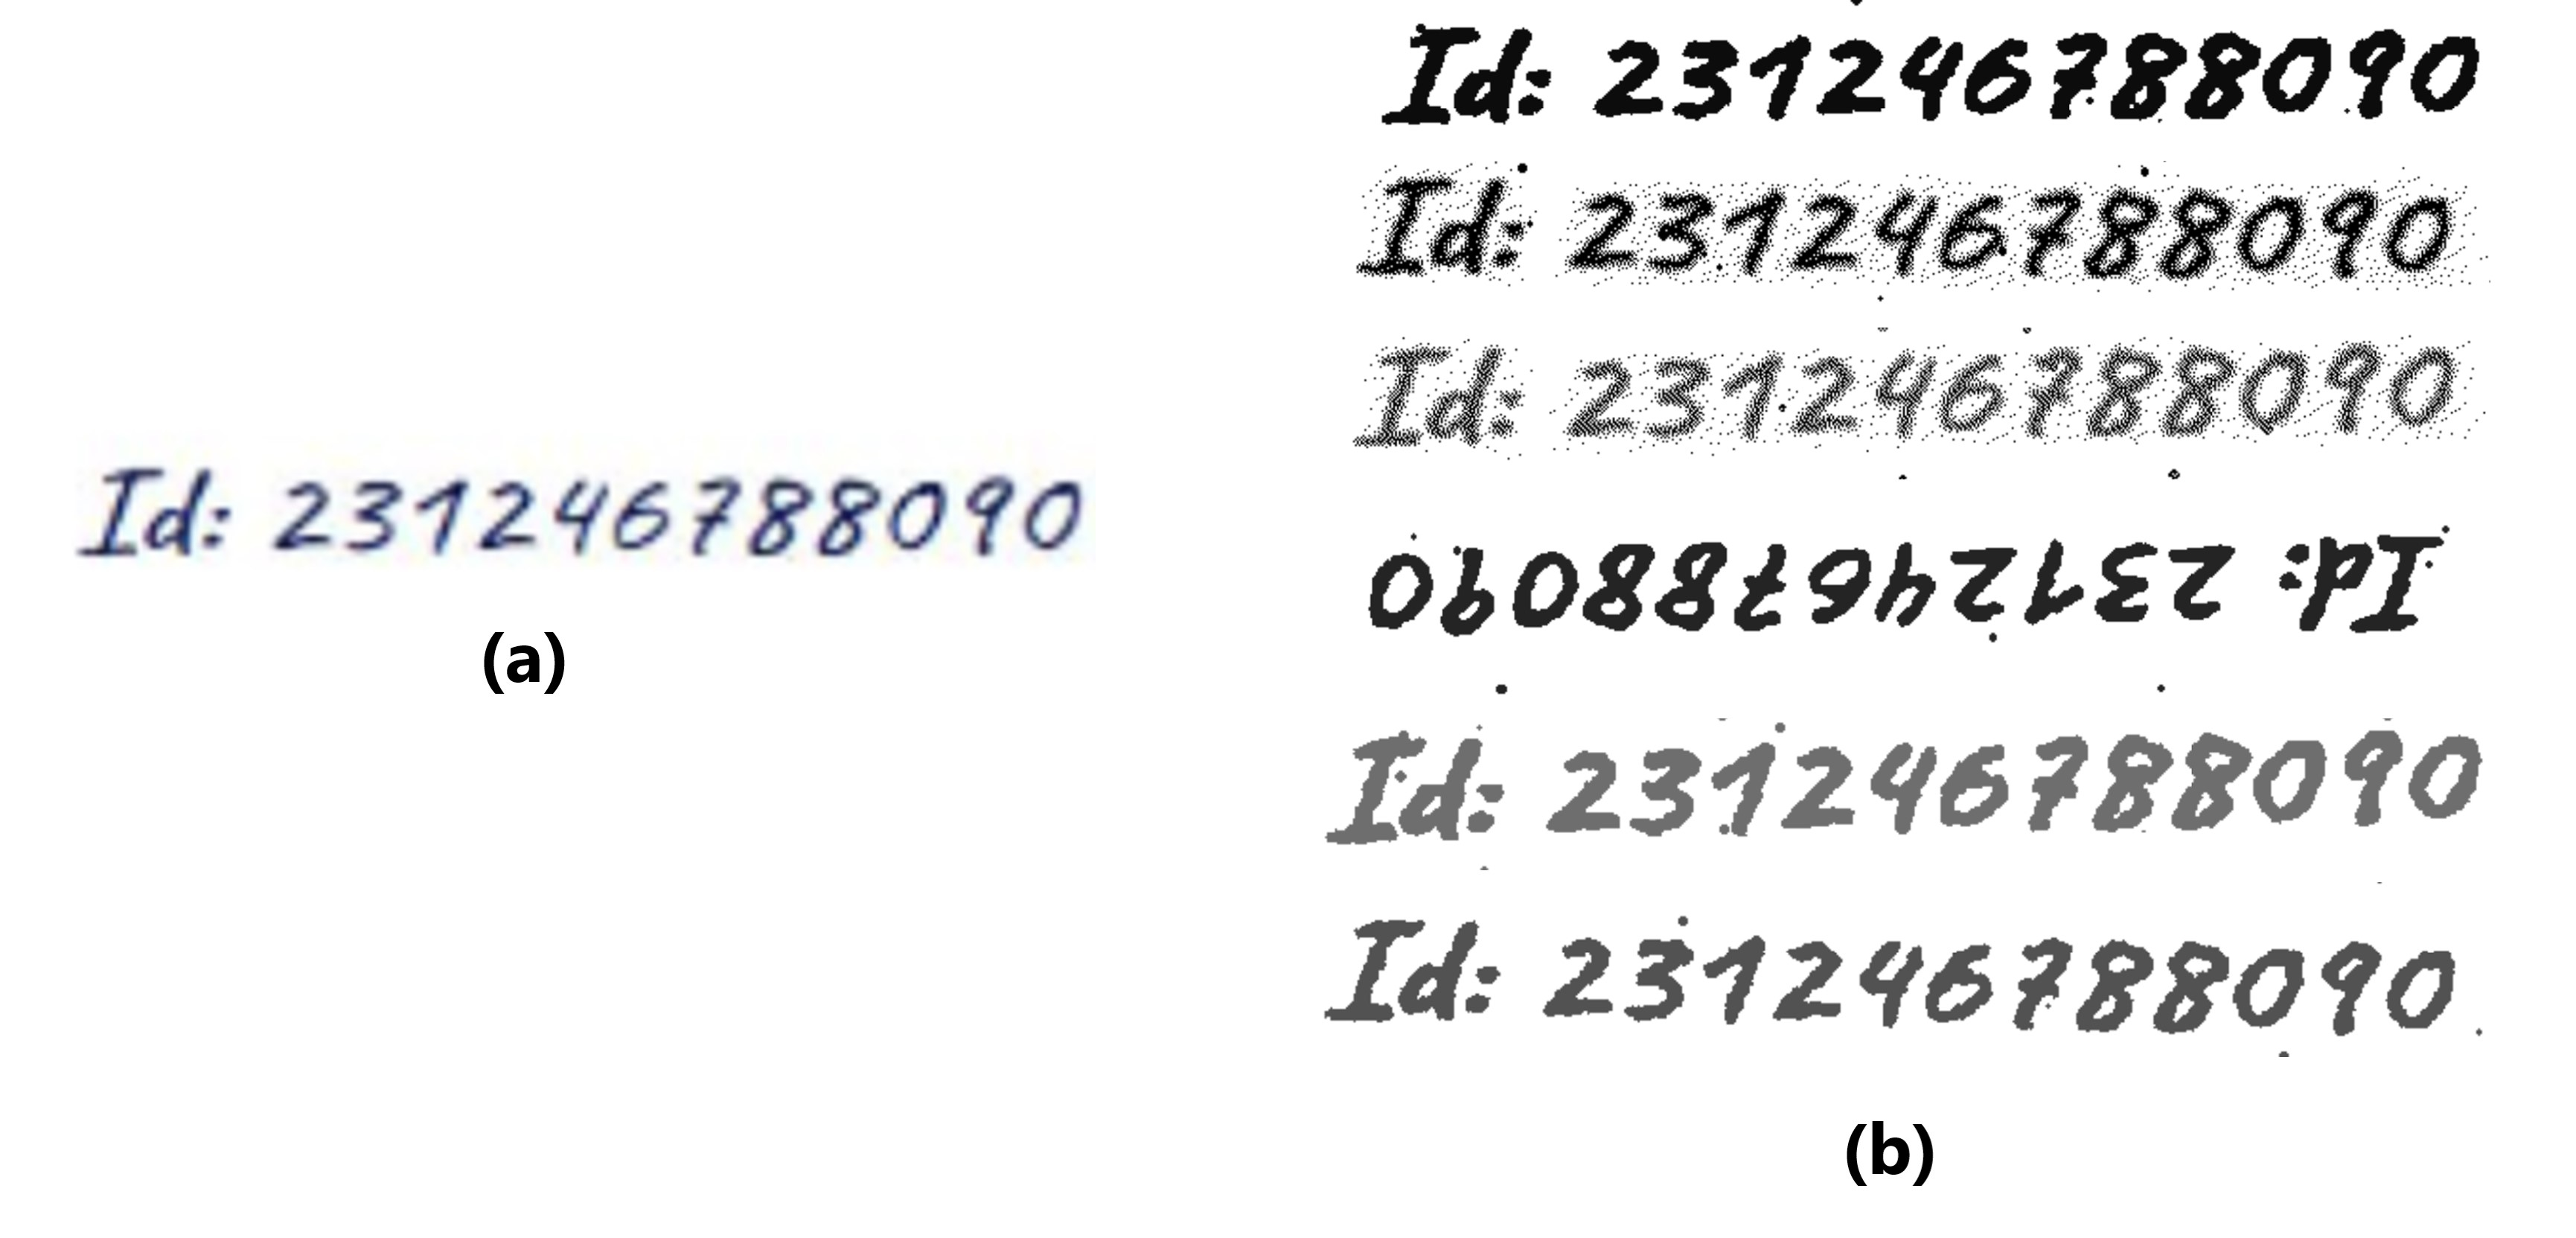
\includegraphics[scale=0.15]{images/Evaluation/FaxificationProcessZoomed.jpg}
	    \caption[Illustration of faxified document images to conclude that faxification process is a random process, the input images are faxified randomly to create distinct output.]{Illustration of faxified document images to conclude that faxification process is a random process, the input images are faxified randomly to create distinct and random output. For example, for a snippet in a synthetic document image (a), snippets of faxified document images shown in (b) are created distinct and random.}
	    \label{fig:FaxificationProcessZoomed}
	    \end{center}
\end{figure}


The faxification process mimics the way the fax machine works. Usually, fax machines transmit only black-and-white images, which might be dirty and are generally also not aligned perfectly. This leads to several common artifacts being introduced into transferred images, so faxification process attempts to mimic those introductions of artifacts into images. The faxification process transforms clean gray-scale synthetic document images in such a way like it was sent via fax. The faxification process is not deterministic, involves randomness during the process of faxification of the images. It uses several image transformations like gamma transformation, brightness transformation, 180-degree rotations, resizing, rescaling, binarization, adding noise, adding verticle lines, and conversion to a grayscale image. The faxification process can be visualized in figure \ref{fig:FaxificationProcess}. In figure \ref{fig:FaxificationProcessZoomed}, it is visible a snippet from the synthetic document image that has transformed randomly into different image transformations when it has been through the faxification process. The faxification process is implemented in Python using a traditional programming approach.

Before this experiment faxified document images dataset is created using synthetic document images and faxification process (figure \ref{fig:FaxificationProcess}). In this experiment, the same classifier (table \ref{table:ClassifierArchitecture}), is trained on faxified document images dataset. The performance of this classifier is evaluated on annotated real document images (test dataset) to understand the domain gap between real data distribution and faxified data distribution. The classification report in table \ref{table:FaxifiedClassificationReport} states that the accuracy of this classifier on annotated real document images is 43\%, macro average f1-score is  58\%, and weighted average f1-score is 43\%. The weighted average f1-score concludes that the faxified data distribution matched more than 40\% to the real data distribution. Also, compared to other data distributions like synthetic and \ac{CycleGAN} generated, the faxified data distribution is more similar to the real data distribution. The confusion matrix is illustrated in figure \ref{fig:CMFaxifiedDocumentImagesClassifier}. In the confusion matrix, it's visible that document images of class DE\_LY\_Bein\_2020-01 are wrongly classified as DE\_LY\_Bein\_2020-03. The rest of the document images are classified satisfactorily. The epochs against accuracy and epochs against loss plots while training classifier on synthetic document images is illustrated in figure \ref{fig:FaxifiedClassifierAcc} and \ref{fig:FaxifiedClassifierLoss} respectively.

\begin{figure}[H]
  \centering
  \begin{minipage}[b]{0.49\textwidth}
    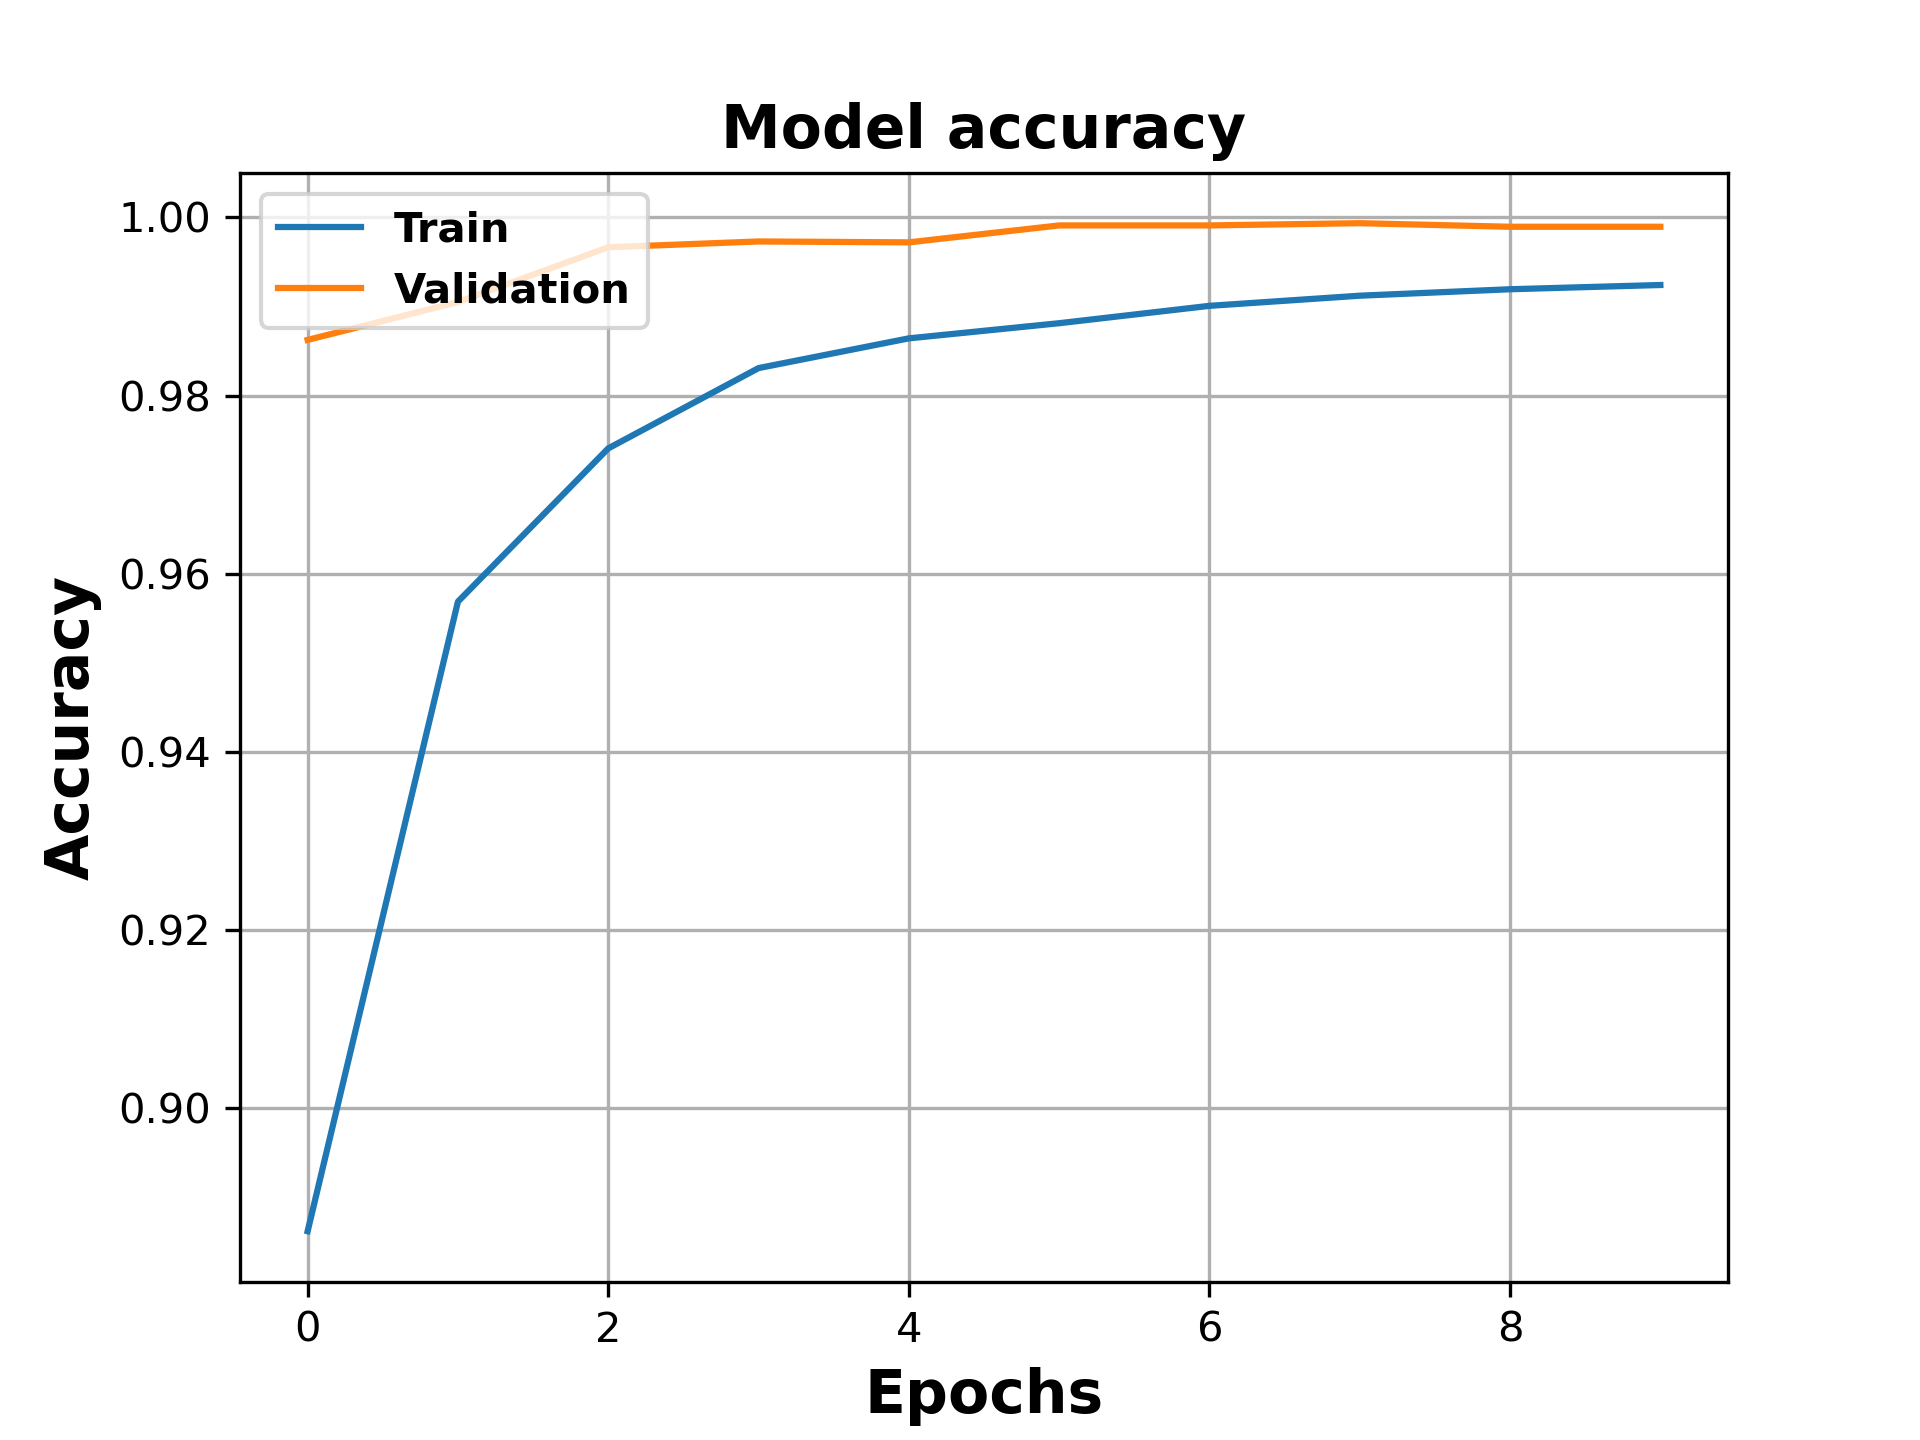
\includegraphics[width=\textwidth]{images/Evaluation/Faxified_Data_Classifier_2021-05-31_19-31-35_Accuracy.png}
    \caption[Epoch vs Accuracy Plot.]{Epoch vs Accuracy Plot.}
    \label{fig:FaxifiedClassifierAcc}
  \end{minipage}
  \hfill
  \begin{minipage}[b]{0.49\textwidth}
    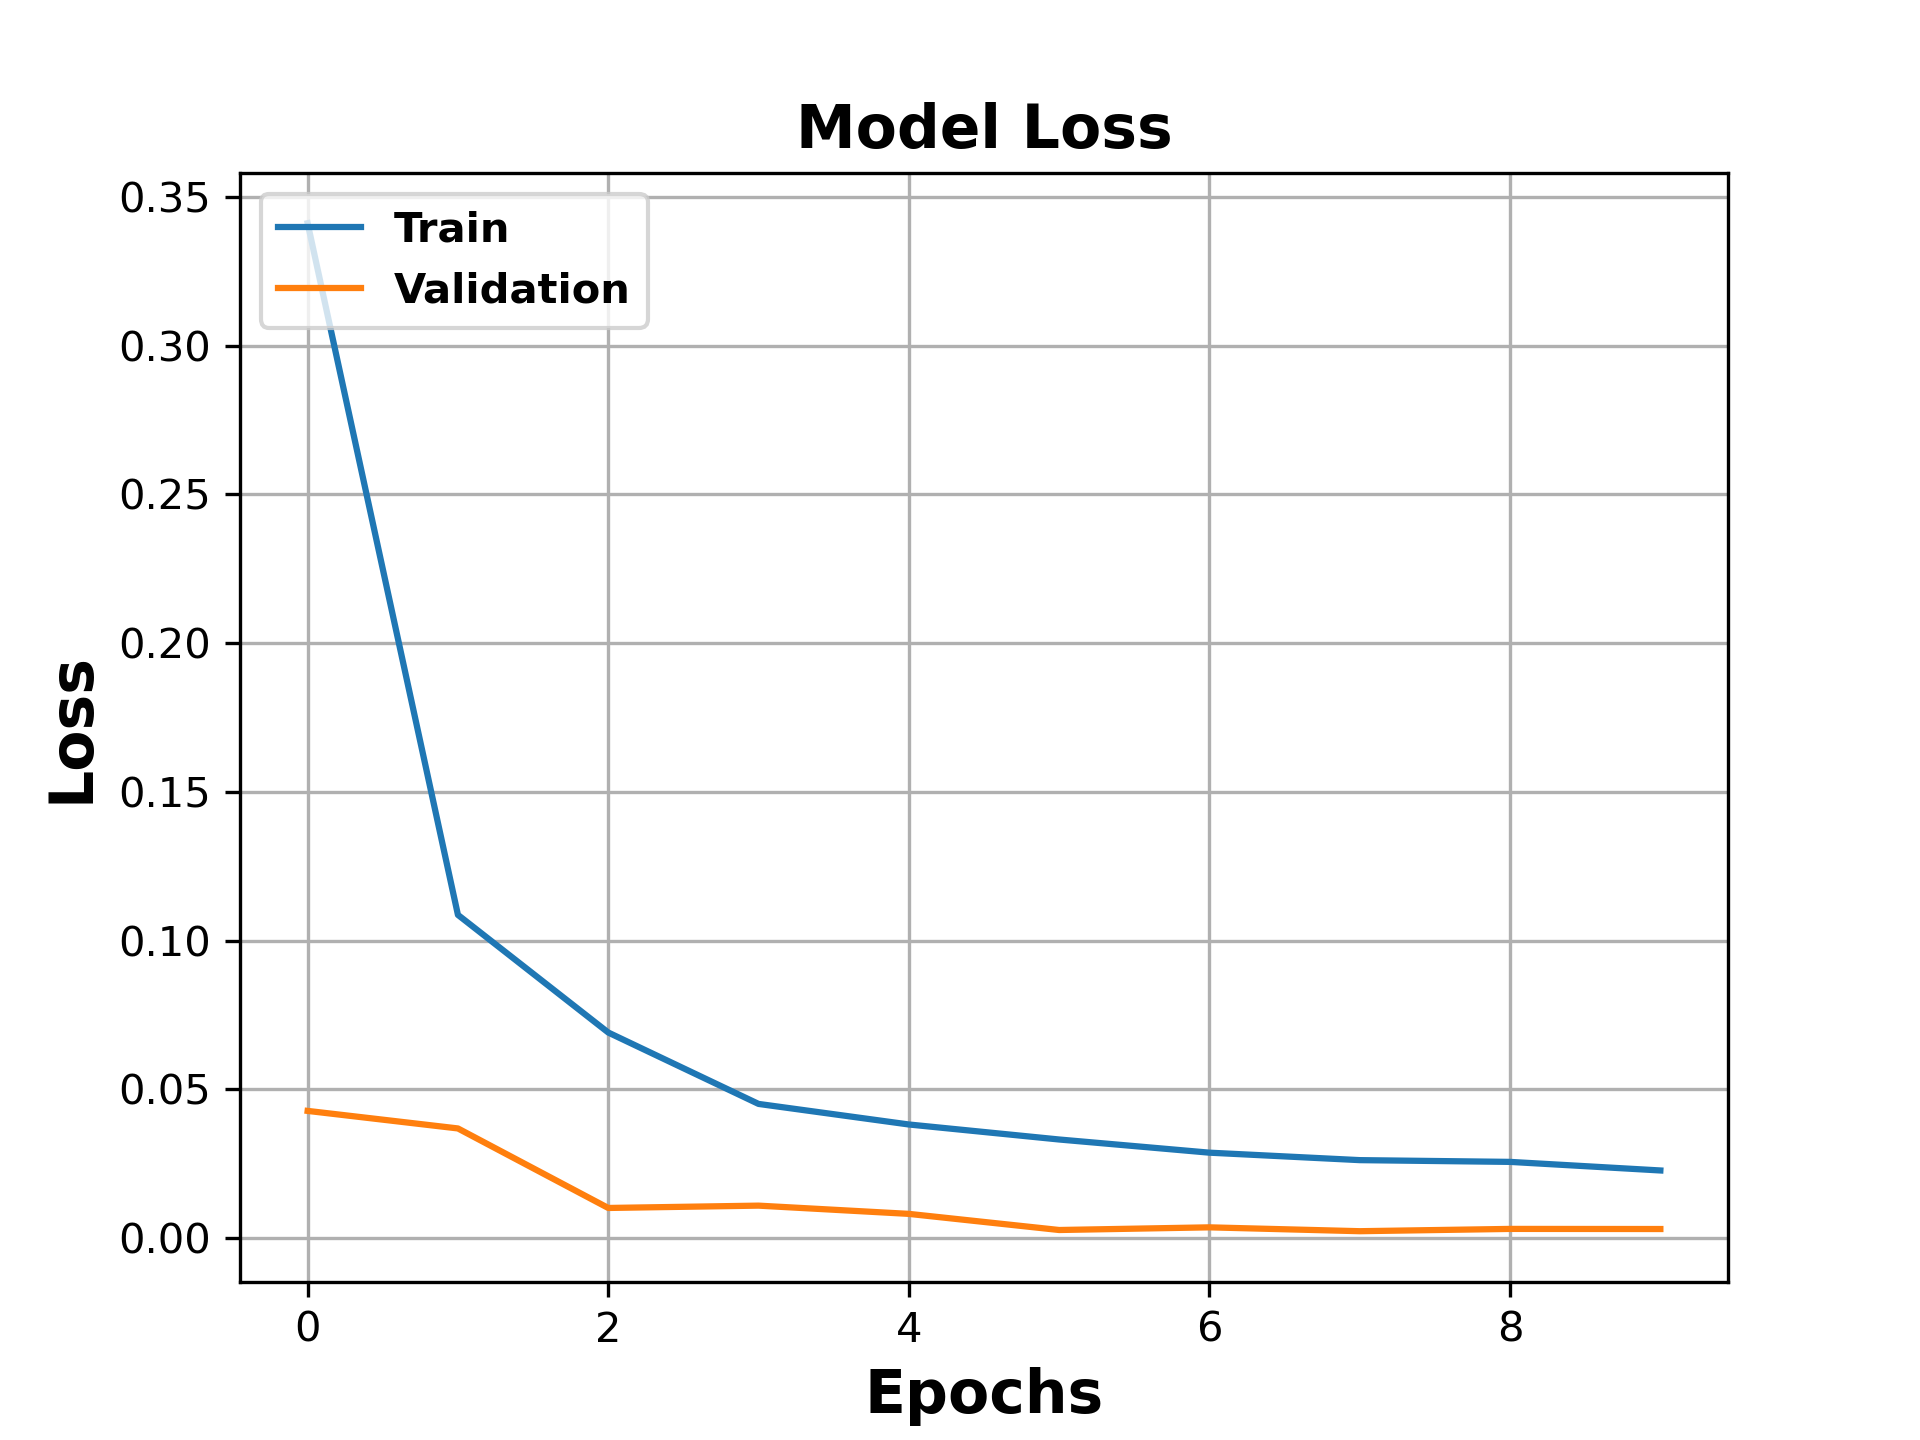
\includegraphics[width=\textwidth]{images/Evaluation/Faxified_Data_Classifier_2021-05-31_19-31-35_Loss.png}
    \caption[Epoch vs Loss Plot.]{Epoch vs Loss Plot.}
    \label{fig:FaxifiedClassifierLoss}
  \end{minipage}
\end{figure}

\begin{center}
\begin{table}[H]
    \begin{center}
    \begin{tabular}{P{0.22\linewidth} P{0.10\linewidth} P{0.10\linewidth} P{0.10\linewidth} P{0.10\linewidth}} 
        \toprule
            & Precision & Recall & f1-score & Support\\[0.0ex] 
        \midrule
        DE\_LY\_Arm\_2020-01 & 0.97 & 0.75 & 0.85 & 44\\[0.0ex]
        \midrule
        DE\_LY\_Bein\_2018-08 & 1.00 & 0.53 & 0.69 & 47\\[0.0ex]
        \midrule
        DE\_LY\_Bein\_2019-01 & 0.74 & 0.34 & 0.47 & 50\\[0.0ex]
        \midrule
        DE\_LY\_Bein\_2019-07 & 0.53 & 1.00 & 0.69 & 60\\[0.0ex]
        \midrule
        DE\_LY\_Bein\_2020-01 & 1.00 & 0.17 & 0.29 & 624\\[0.0ex]
        \midrule
        DE\_LY\_Bein\_2020-03 & 0.19 & 0.98 & 0.32 & 128\\[0.0ex]
        \midrule
        DE\_LY\_Hand\_2020-01 & 0.21 & 1.00 & 0.34 & 16\\[0.0ex]
        \midrule
        DE\_PH\_Bein\_2018-09 & 0.68 & 0.68 & 0.68 & 22\\[0.0ex]
        \midrule
        DE\_PH\_Bein\_2019-02 & 0.78 & 0.64 & 0.71 & 28\\[0.0ex]
        \midrule
        DE\_PH\_Bein\_2020-01 & 1.00 & 0.59 & 0.74 & 143\\[0.0ex]
        \midrule
        \midrule
        Accuracy              &      &      & \bf{0.43} & 1162\\[0.0ex]
        Macro average             & 0.71 & 0.67 & \bf{0.58} & 1162\\[0.0ex]
        Weighted average          & 0.85 & 0.43 & \bf{0.43} & 1162\\[0.0ex]

        \bottomrule
    \end{tabular}
    \caption[Classification report generated after the classifier is trained on faxified document images, its classification performance evaluated on the annotated real document images.]{Classification report generated after the classifier is trained on faxified document images, its classification performance evaluated on the annotated real document images.}
    \label{table:FaxifiedClassificationReport}
    \end{center}
\end{table}
\end{center}



















\section{Results}\label{results}
In this chapter, the qualitative and quantitative results are discussed. In section \ref{QualitativeResults}, the qualitative results are illustrated to understand the quality of \ac{CycleGAN} generated document images. Also, the typical failure cases of the proposed method to the problem statement are illustrated in section \ref{FailureCases}. In figure \ref{fig:QualitativeResults}, some images of synthetic document images that are transformed into realistic document images by the proposed image-to-image translation application are illustrated. The figure \ref{fig:failure1} illustrates the proposed image-to-image translation application using \ac{CycleGAN} has failed to transform handwritten crops present in the synthetic document images. The figure \ref{fig:failure2} illustrates the transformed image has undesired noisy artifacts. Figure \ref{fig:failure3} illustrates transformed image has a dark border and noisy artifacts. Figure \ref{fig:failure4} illustrates transformed image has random artifacts that are not present in the synthetic document image.


\subsection{Quantitative Results}\label{QuantitativeResults}


\hspace*{5.0em}

\begin{table}[H]
%\hspace*{-5.40em}
\begin{tabular}{P{0.25\linewidth} P{0.20\linewidth} P{0.20\linewidth} P{0.20\linewidth}} 
	\toprule
	\bf{Data distributions} & \bf{Accuracy}  & \bf{Weighted average f1-score} & \bf{Macro average f1-score} \\[0.0ex] 
	\midrule
     \bf{Synthetic document images} & 25\% & 31\% & 27\%\\[0.0ex]
     \midrule
     \bf{\ac{CycleGAN} generated document images} & 27\% & 25\% & 34\%\\[0.0ex]
     \midrule
     \bf{Faxified document images} & 43\% & 43\% & 58\%\\[0.0ex]
     \bottomrule
\end{tabular}
 \caption[The accuracies and f1-scores when the classifiers trained on different data distributions and evaluated on annotated real document images.]{The accuracies and f1-scores when the classifiers trained on different data distributions and evaluated on annotated real document images.}
    \label{table:finalResults}
\end{table}


\begin{figure}[H]
        \begin{center}
	    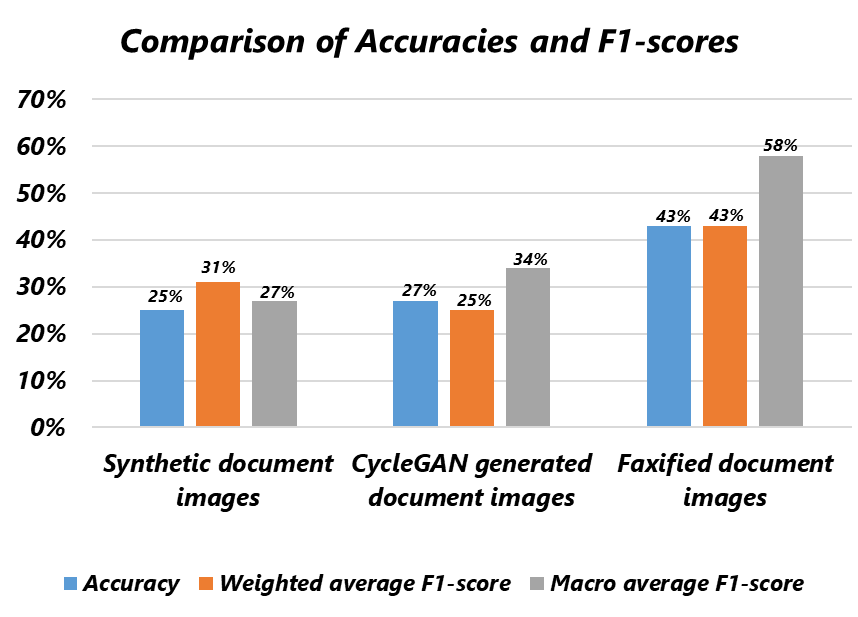
\includegraphics[scale=0.90]{images/Evaluation/ComparisonOfAccuracyAndF1Score.png}
	    \caption[Comparison of accuracies and f1-scores, when the classifiers trained on different data distributions and evaluated on annotated real document images.]{Comparison of accuracies and f1-scores, when the classifiers trained on different data distributions and evaluated on annotated real document images.}
	    \label{fig:ComparisonOfAccuracyAndF1Score}
	    \end{center}
\end{figure}


\subsection{Qualitative Results}\label{QualitativeResults}


\begin{figure}[H]
        \begin{center}
	    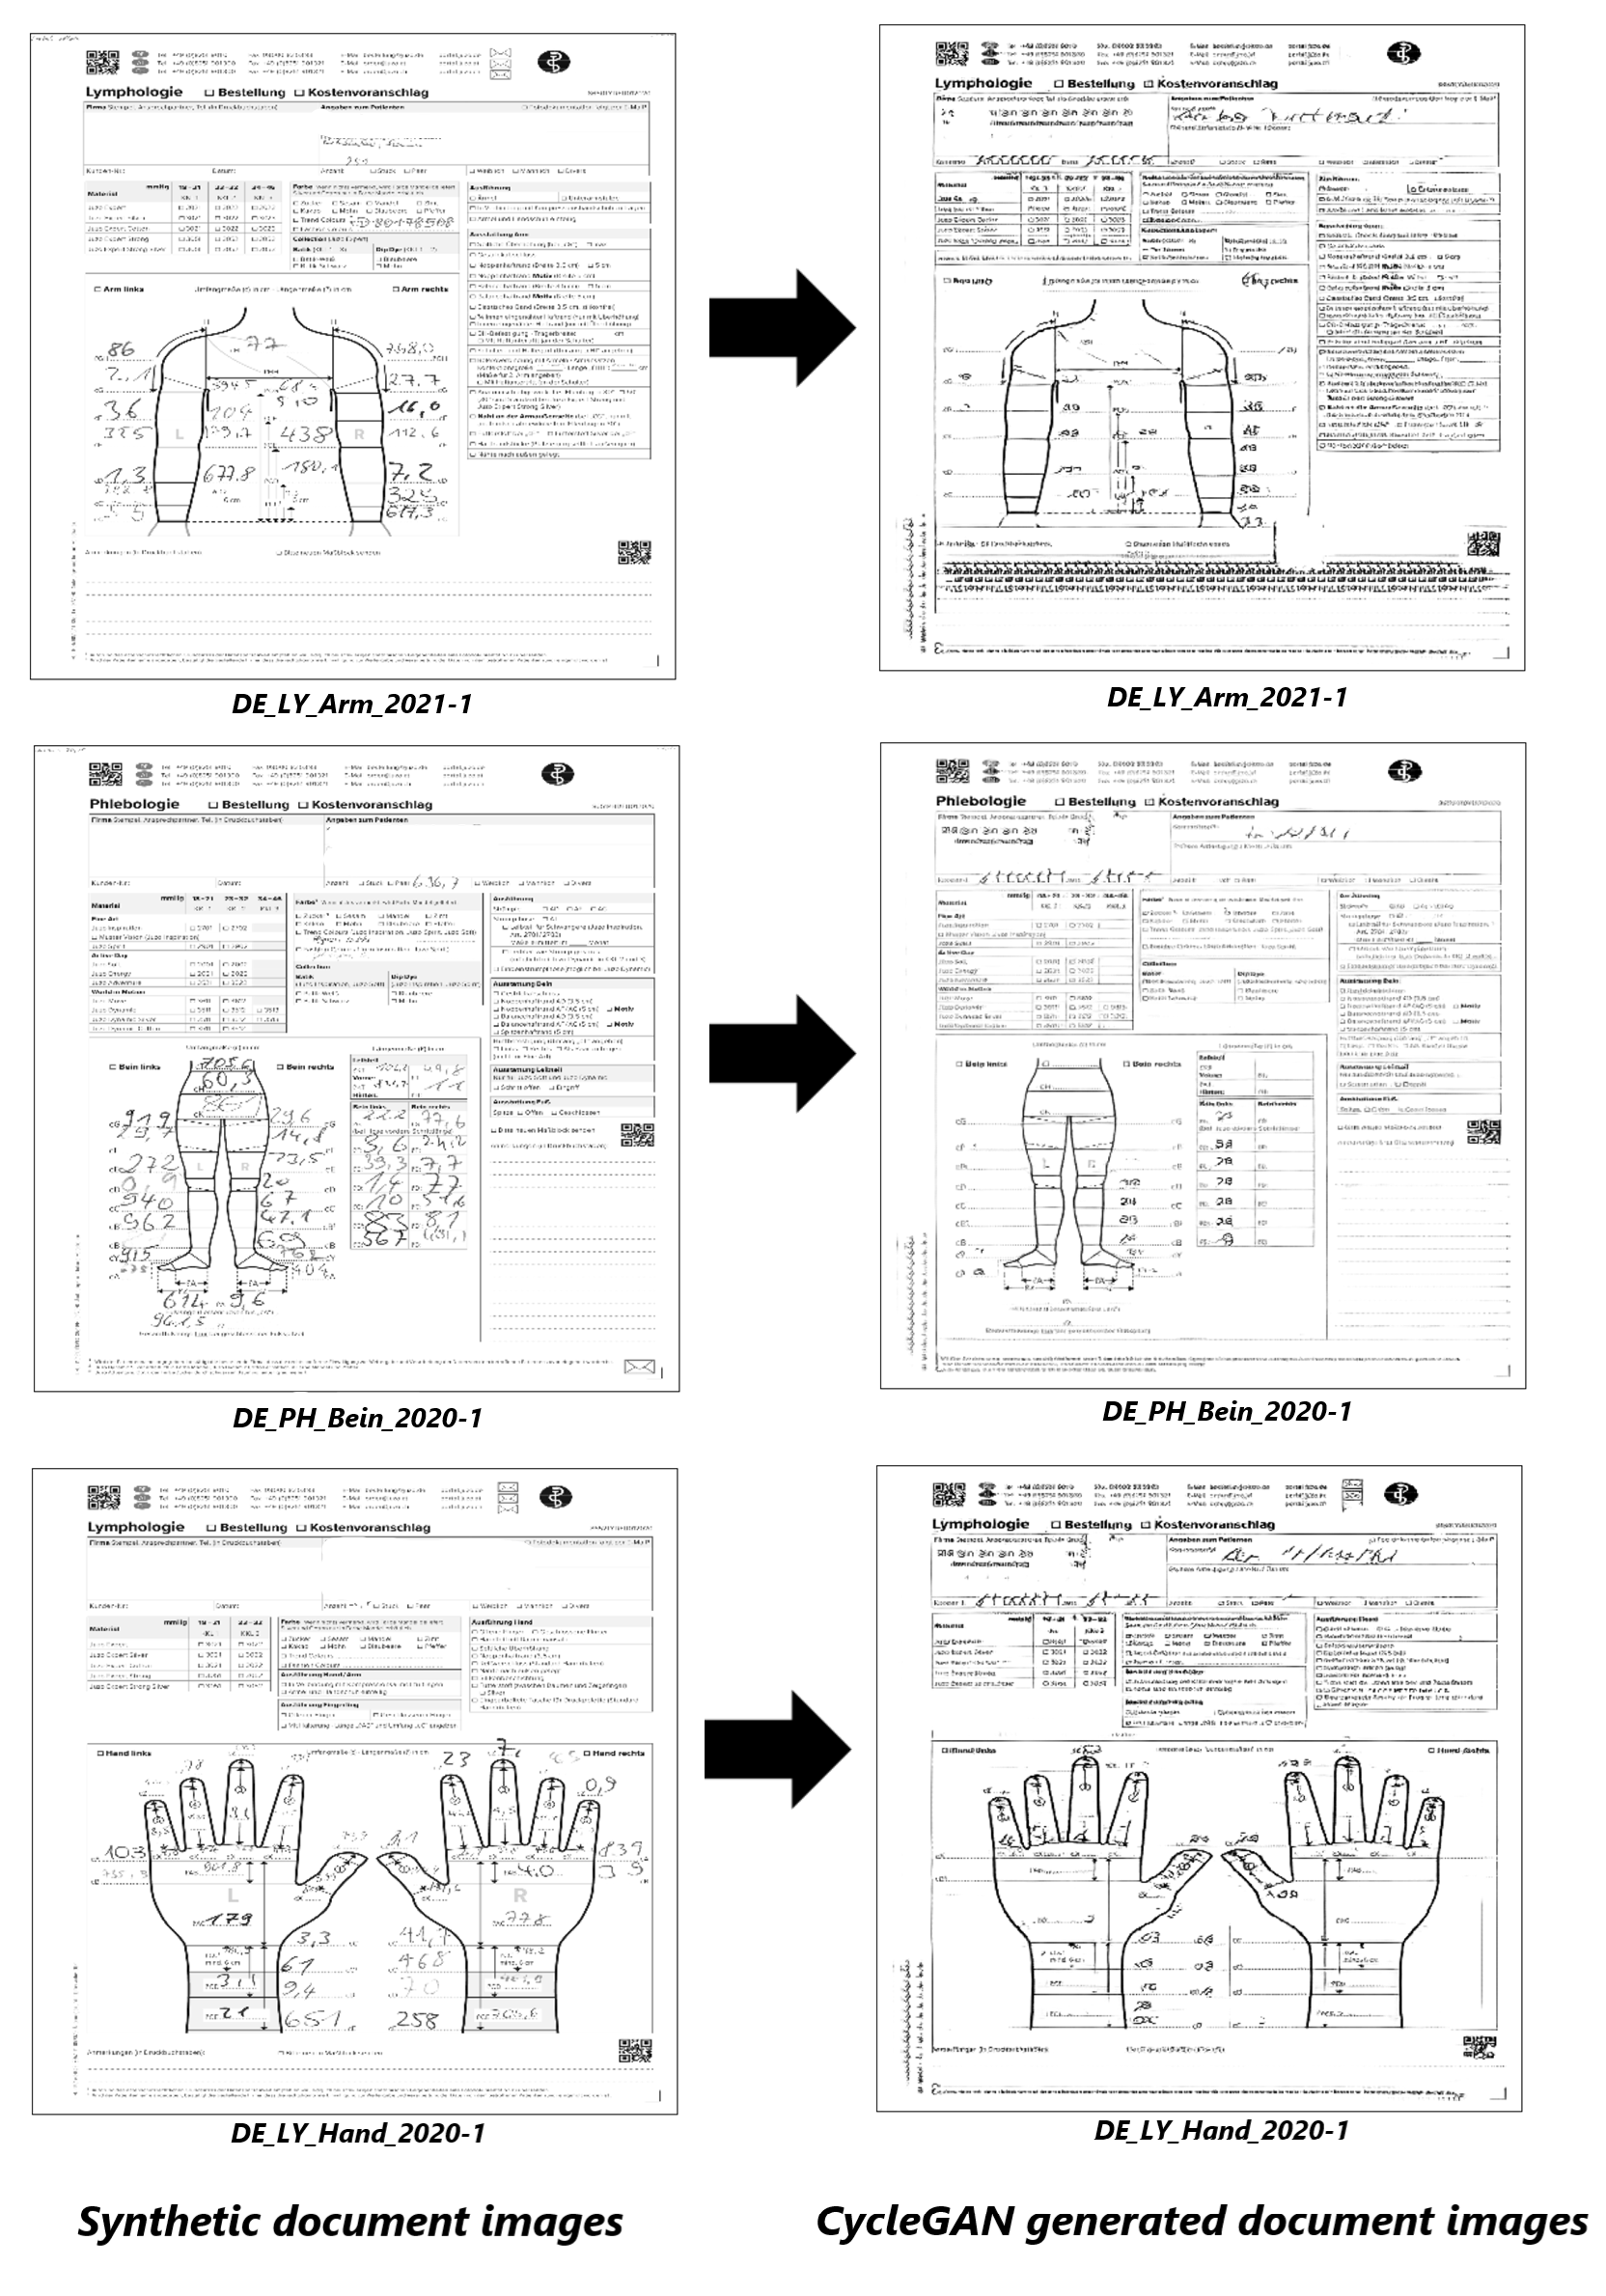
\includegraphics[scale=0.30]{images/Evaluation/Qualitative_Results.png}
	    \caption[Synthetic document images transformed into realistic document images by the image-to-image translation application.]{Synthetic document images transformed into realistic document images by the image-to-image translation application (figure reproduced from elevait GmbH \& Co. KG with permission).}
	    \label{fig:QualitativeResults}
	    \end{center}
\end{figure}


In section \ref{QuantitativeResults}, the quantitative results are illustrated using a table and bar plot. In which the performance of the classifier trained using different distributions is evaluated and compared. The evaluation metrics like accuracy, macro average f1-score, and weighted average f1-score are used. As the testing dataset of annotated real document images is unbalanced we consider weighted average f1-score for comparison. Results show the \ac{CycleGAN} generated document images were 25\% similar to the real document images. But, the faxified document images were 43\% similar to the real document images. Results reveal that \ac{CycleGAN} could not achieve the expected results quantitatively. The faxified data distribution created using the faxification process was satisfactorily matched to the real data distribution. The qualitative results (figure \ref{QualitativeResults}) look very promising. The proposed image-to-image translation application can be improved further in the future using different methods and loss functions. The future work and discussion about the results achieved in this thesis are explained in the chapter \ref{conclusion} in more detail.



\subsection{Failure Cases}\label{FailureCases}

\begin{figure}[H]
        \begin{center}
	    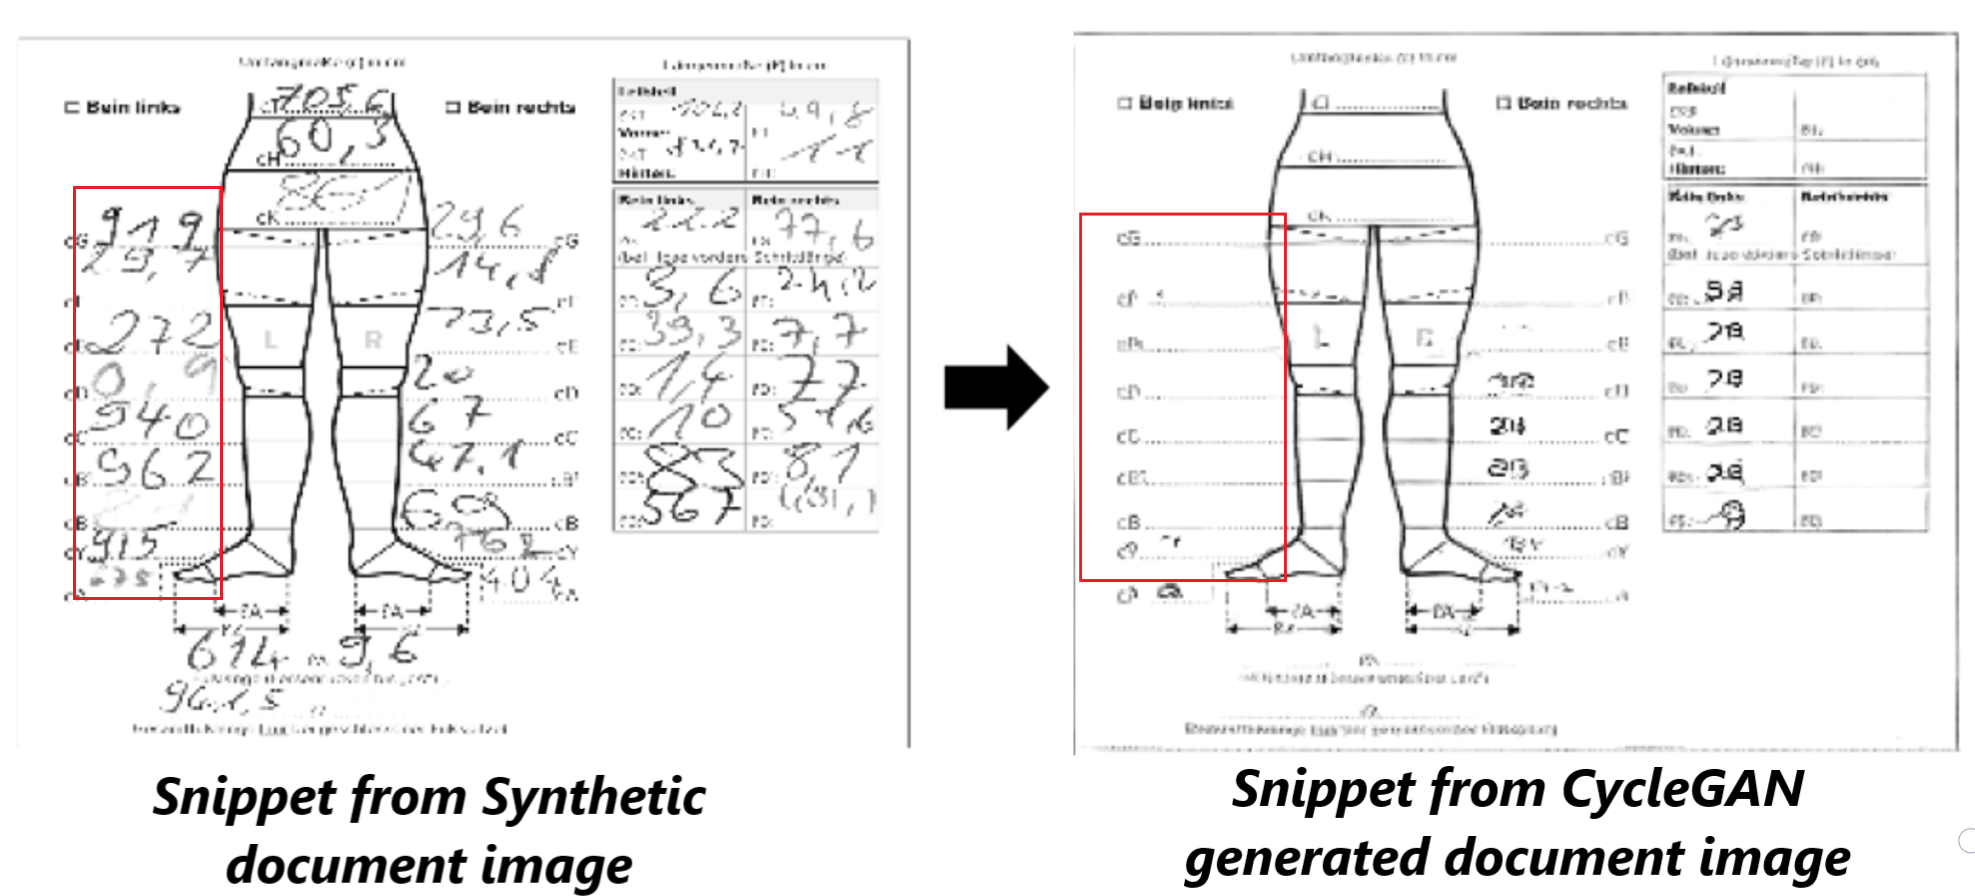
\includegraphics[scale=0.28]{images/Evaluation/failure1.png}
	    \caption[The snippet from \ac{CycleGAN} generated document image illustrates that the proposed image-to-image translation application did not transform or reconstruct handwritten crops in the target domain from the synthetic document image in the source domain.]{The snippet from \ac{CycleGAN} generated document image illustrates that the proposed image-to-image translation application did not transform or reconstruct handwritten crops in the target domain from the synthetic document image in the source domain (figure reproduced from elevait GmbH \& Co. KG with permission).}
	    \label{fig:failure1}
	    \end{center}
\end{figure}

\begin{figure}[H]
        \begin{center}
	    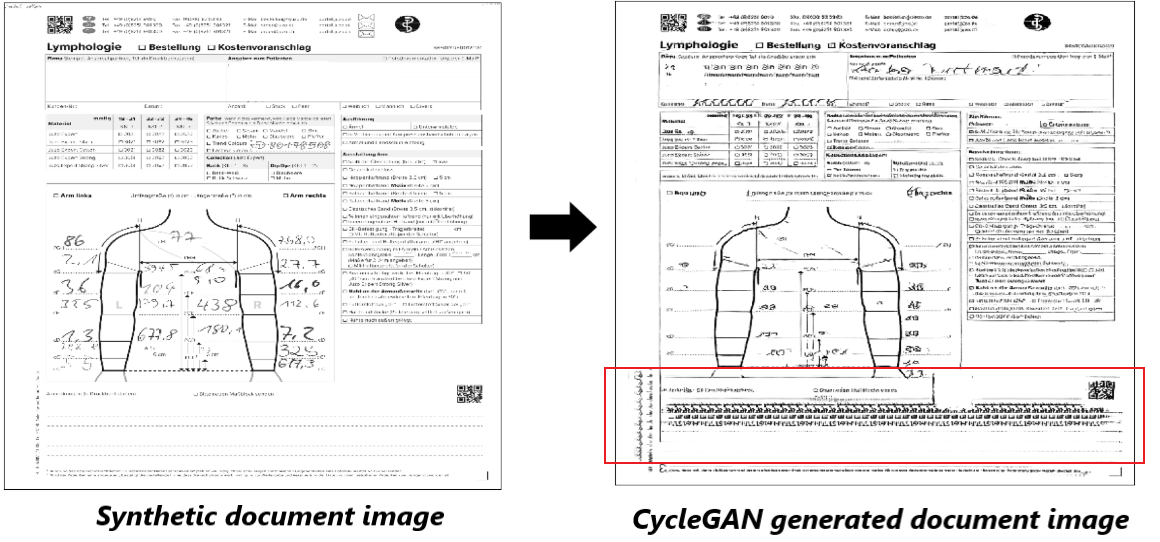
\includegraphics[scale=0.50]{images/Evaluation/failure2.png}
	    \caption[The \ac{CycleGAN} generated document image consists of noisy artifacts that are unrealistic.]{The \ac{CycleGAN} generated document image consists of noisy artifacts that are unrealistic (figure reproduced from elevait GmbH \& Co. KG with permission).}
	    \label{fig:failure2}
	    \end{center}
\end{figure}

\begin{figure}[H]
        \begin{center}
	    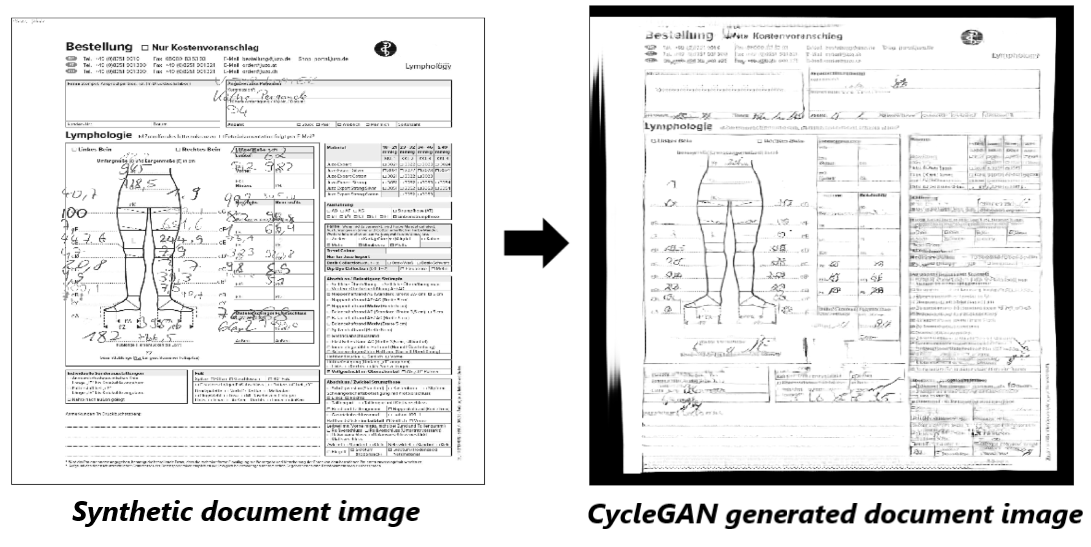
\includegraphics[scale=0.50]{images/Evaluation/failure3.png}
	    \caption[The \ac{CycleGAN} generated document image consists of dark border.]{The \ac{CycleGAN} generated document image consists of dark border (figure reproduced from elevait GmbH \& Co. KG with permission).}
	    \label{fig:failure3}
	    \end{center}
\end{figure}


\begin{figure}[H]
        \begin{center}
	    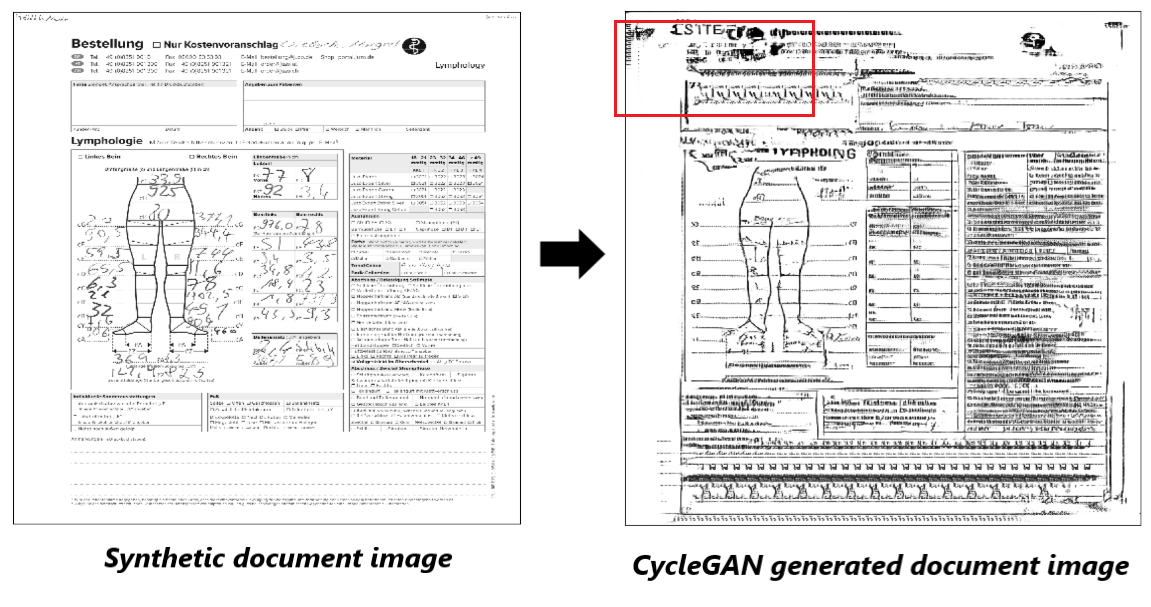
\includegraphics[scale=0.50]{images/Evaluation/failure4.png}
	    \caption[There are some artifacts appear in the generated image that are not present in the synthetic image.]{The \ac{CycleGAN} generated document image consists of noisy artifacts that are unrealistic and the visual quality of the generated image is not good. There are some artifacts (marked in red box) appear in the generated images that are not present in the synthetic image (figure reproduced from elevait GmbH \& Co. KG with permission).}
	    \label{fig:failure4}
	    \end{center}
\end{figure}




































%%%%%%%%%%%%%%%%%%%%%%%%%%%%%%%%%%%%%%%%%%%%%%%%%%%%%%%%%%%%%%%%%%%%%%%%%%%%%%%%%%%%%%%%%%%%%%%%%%%%%%%%%%%%%%%%%%%

%\subsection{Overview of Domain Gap between Distribution}
\begin{comment}
\begin{figure}[H]
        \begin{center}
	    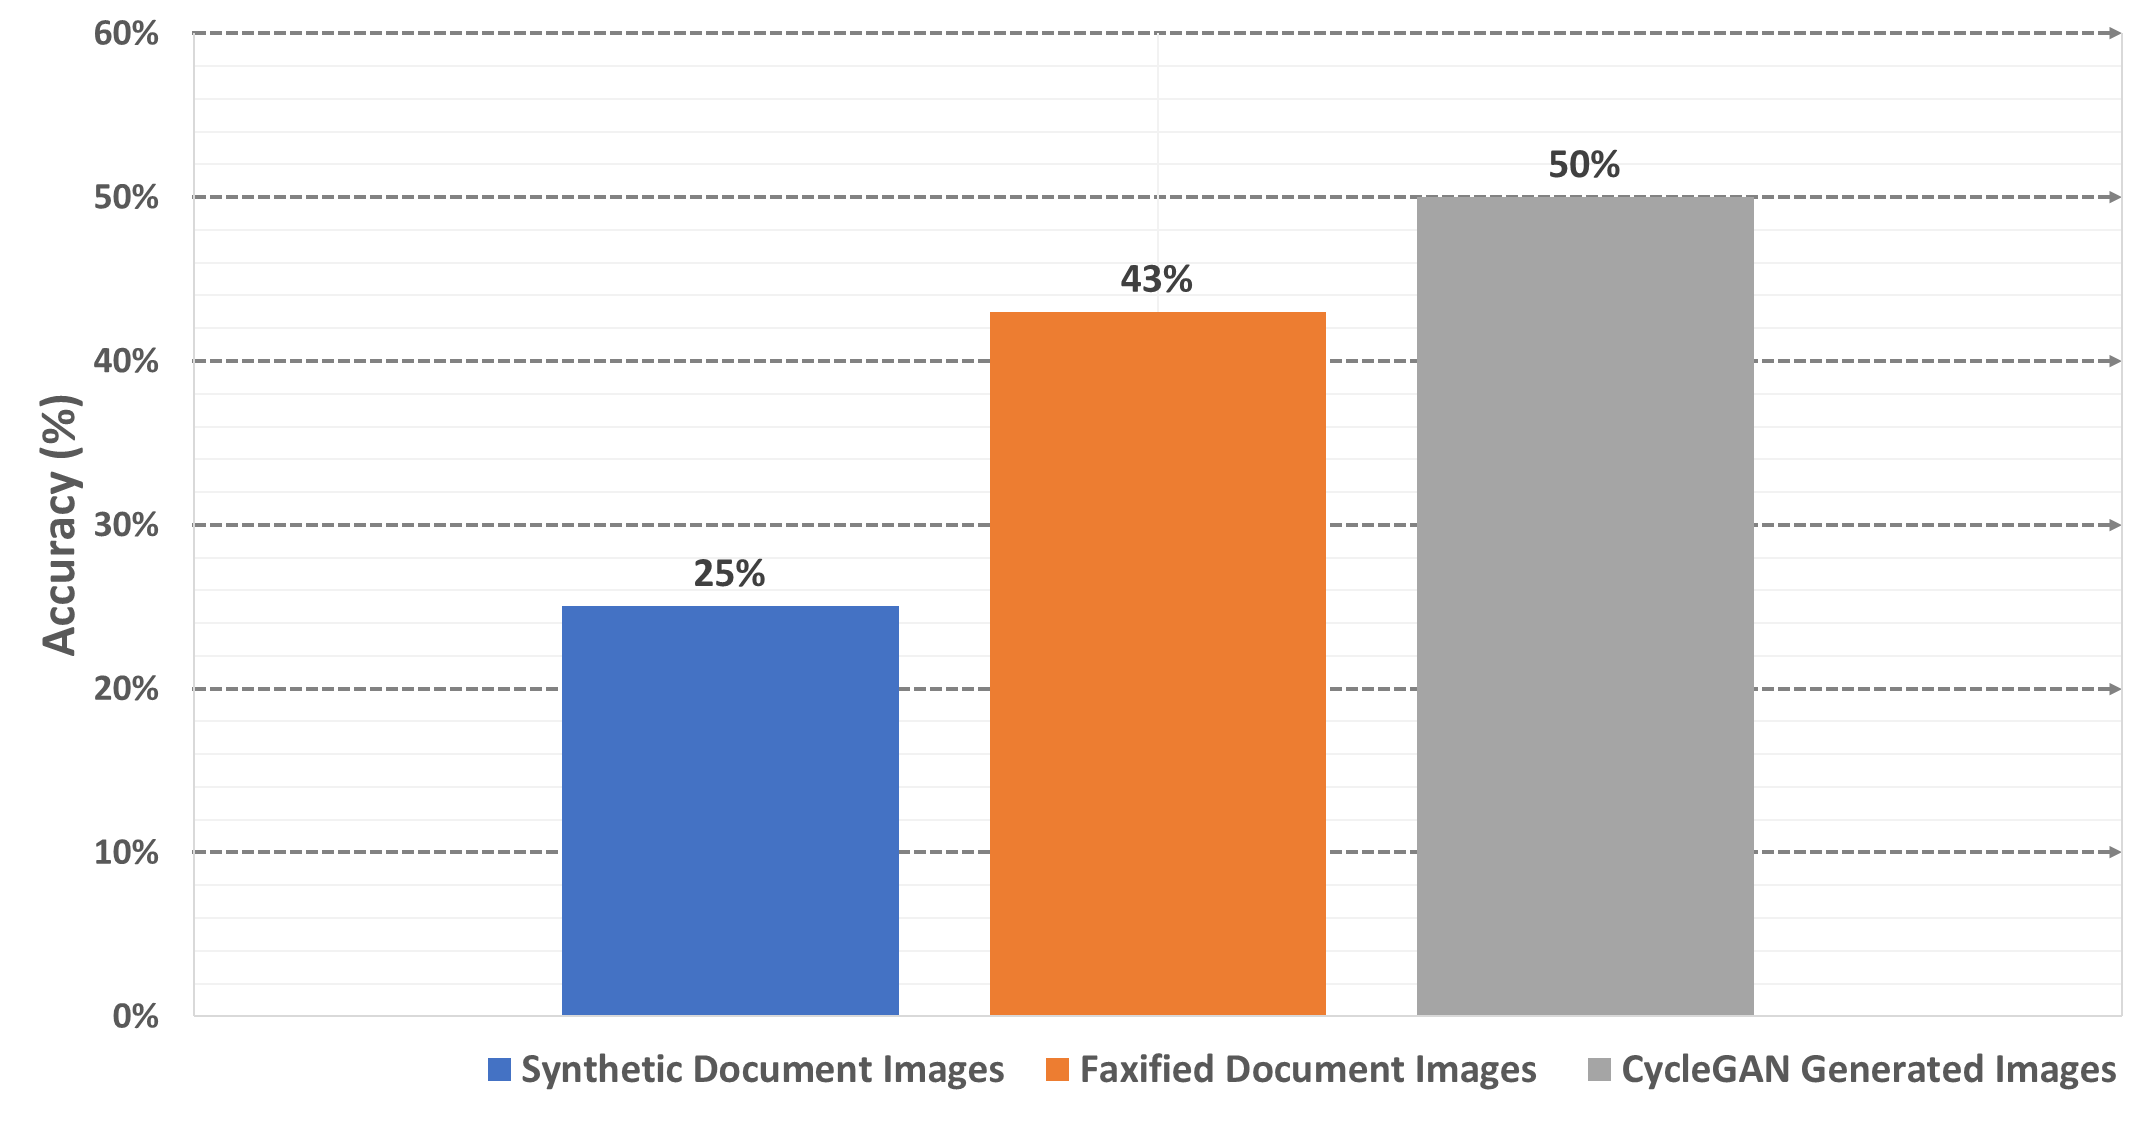
\includegraphics[scale=0.20]{images/DomainGap.png}
	    \caption[Illustration of Domain Gap Between Real Data Distribution and Synthetic Data Distribution, Faxified Data Distribution, and \ac{CycleGAN} Generated Data Distribution.]{Illustration of Domain Gap Between Real Data Distribution and Synthetic Data Distribution, Faxified Data Distribution, and \ac{CycleGAN} Generated Data Distribution. Initially, the classifiers are trained on Synthetic Document Images, Faxified Document Images, and \ac{CycleGAN} Generated Document Images. Later their Classification Performance Evaluated on the Annotated Real Document Images to understand the Domain Gap between distributions using Accuracy as an Evaluation Metric.}
	    \label{fig:DomainGap}
	    \end{center}
\end{figure}
\end{comment}

%To evaluate the quality of images generated by the \ac{CycleGAN}, a classifier is trained on the \ac{CycleGAN} generated data and its accuracy on a real dtest dataset is used as a metric to measure how well the \ac{CycleGAN} model distribution matches the real data distribution. Basically, The classification capability of the trained classifier is used as an objective measure to assess the quality of images generated by \ac{CycleGAN}. Also, the classifier is trained on the synthetic document images and it's accuracy evaluated in 
%Classification report and metrics
%Three separate classifiers are trained upon synthetic data distribution, faxified data distribution, and \ac{CycleGAN} generated data distribution respectively. After training the classifiers they have evaluated annotated real document images. Using this performance evaluation using metrics like weighted f1 score and accuracy 	


\begin{comment}
\begin{center}
\begin{table}[H]
    \begin{center}
    \begin{tabular}{P{0.30\linewidth} P{0.15\linewidth} P{0.20\linewidth} P{0.20\linewidth}} 
        \toprule
        \bf{Data Distributions} & \bf{Accuracy}  & \bf{Weighted average f1-score} & \bf{Macro average f1-score} \\[0.0ex] 
        \midrule
        \bf{Synthetic document images} & 25\% & 31\% & 27\%\\[0.0ex]
        \midrule
       \bf{\ac{CycleGAN} generated document images} & 27\% & 47\% &34\%\\[0.0ex]
        \midrule
        \bf{Faxified document images} & 43\% & 43\% & 58\%\\[0.0ex]
        \bottomrule
    \end{tabular}
    \caption[Comparison of accuracy and f1-scores when the classifiers trained on different data distributions and evaluated on annotated real document images.]{Comparison of accuracy and f1-scores when the classifiers trained on different data distributions and evaluated on annotated real document images.}
    \label{table:finalResults}
    \end{center}
\end{table}
\end{center}




\begin{center}
\begin{table}[H]
    \begin{center}
    \begin{tabular}{P{0.22\linewidth} P{0.22\linewidth} P{0.22\linewidth} P{0.22\linewidth}} 
        \toprule
        \bf{Classifier trained using} & \bf{Accuracy on annotated real document images}  & \bf{Weighted average f1-score on annotated real document images} & \bf{Macro average f1-score on annotated real document images} \\[0.0ex] 
        \midrule
        \bf{Synthetic document images} & 25\% & 31\% & 27\%\\[0.0ex]
        \midrule
       \bf{\ac{CycleGAN} generated document images} & 27\% & 47\% &34\%\\[0.0ex]
        \midrule
        \bf{Faxified document images} & 43\% & 43\% & 58\%\\[0.0ex]
        \bottomrule
    \end{tabular}
    \caption[Comparison of accuracy and f1-scores when the classifiers trained on different data distributions and evaluated on annotated real document images.]{Comparison of accuracy and f1-scores when the classifiers trained on different data distributions and evaluated on annotated real document images.}
    \label{table:finalResults}
    \end{center}
\end{table}
\end{center}



\begin{center}
\begin{table}[H]
    \begin{center}
    \begin{tabular}{P{0.35\linewidth} P{0.12\linewidth} P{0.20\linewidth} P{0.20\linewidth}} 
        \toprule
        \bf{Data distributions} & \bf{Accuracy}  & \bf{Weighted average f1-score} & \bf{Macro average f1-score} \\[0.0ex] 
	 \midrule
        \bf{Synthetic document images} & 25\% & 31\% & 27\%\\[0.0ex]
        \midrule
       \bf{\ac{CycleGAN} generated document images} & 27\% & 25\% & 34\%\\[0.0ex]
        \midrule
        \bf{Faxified document images} & 43\% & 43\% & 58\%\\[0.0ex]
        \bottomrule
    \end{tabular}
    \caption[Comparison of accuracy and f1-scores when the classifiers trained on different data distributions and evaluated on annotated real document images.]{Comparison of accuracy and f1-scores when the classifiers trained on different data distributions and evaluated on annotated real document images.}
    \label{table:finalResults}
    \end{center}
\end{table}
\end{center}

\begin{table}[H]
\hspace*{-5.40em}
\begin{tabular}{cccc} 
	\toprule
	\bf{Data distributions} & \bf{Accuracy}  & \bf{Weighted average f1-score} & \bf{Macro average f1-score} \\[0.0ex] 
	\midrule
     \bf{Synthetic document images} & 25\% & 31\% & 27\%\\[0.0ex]
     \midrule
     \bf{\ac{CycleGAN} generated document images} & 27\% & 25\% & 34\%\\[0.0ex]
     \midrule
     \bf{Faxified document images} & 43\% & 43\% & 58\%\\[0.0ex]
     \bottomrule
\end{tabular}
 \caption[The accuracies and f1-scores when the classifiers trained on different data distributions and evaluated on annotated real document images.]{The accuracies and f1-scores when the classifiers trained on different data distributions and evaluated on annotated real document images.}
    \label{table:finalResults}
\end{table}


\end{comment}